\subsection{REPRESENTATIONS}

DEFINITION 1. Let \(\mathfrak{g}\) be a Lie algebra over \(\mathbf{K}\) and \(\mathbf{M}\) a \(\mathbf{K}\) -module. A homomorphism of \(\mathfrak{g}\) into the Lie Algebra \(\mathfrak{gl}(\mathbf{M})\) is called a representation of \(\mathfrak{g}\) on the module \(\mathbf{M}\) . An injective representation is called faithful. If \(\mathbf{K}\) is a field, the dimension (finite or infinite) of \(\mathbf{M}\) over \(\mathbf{K}\) is called the dimension of the representation. The representation \(x \mapsto \operatorname{ad} x\) of \(\mathfrak{g}\) on the \(\mathbf{K}\) -module \(\mathfrak{g}\) is called the adjoint representation of \(\mathfrak{g}\) .

A representation of g on M is thus a K-linear mapping \(\rho\) of g into the endomorphism module of M such that

\[
\rho ([ x, y ]). m = \rho (x) \rho (y). m - \rho (y) \rho (x). m
\]

for all \(x \in g, y \in g, m \in M.\)

*Example. Let G be a real Lie group, g its Lie algebra and \(\rho\) an analytic representation of G on a finite-dimensional real vector space E. Then the corresponding homomorphism of g into gl(E) is a representation of g on E.*

Let \(\mathbf{U}\) be the enveloping algebra of \(\mathfrak{g}\) . Proposition 1 of §2, no. 1 defines a one-to-one correspondence between the set of representations of \(\mathfrak{g}\) on \(\mathbf{M}\) and the set of representations of \(\mathbf{U}\) on \(\mathbf{M}\) . On the other hand we know (Algebra, Chapter VIII, §13, no. 1) that there is an equivalence between the notion of representation of the associative algebra \(\mathbf{U}\) and that of left \(\mathbf{U}\) -module.

DEFINITION 2. Let g be a Lie algebra over K and U its enveloping algebra. A unitary left module over U is called a left g-module, or simply a g-module.

If M is a g-module and \(x \in U\) , \(x_{M}\) will denote the homothety of M defined by x (cf.~Algebra, Chapter VIII, § 1, no. 2).

A unitary right module over U is called a right g-module. Such a module is identified with a left \(U^{0}\) -module, that is (§2, no. 4) with a left \(g^{0}\) -module.

Let \(\phi\) be the principal antiautomorphism of U. If M is a right g-module, a left g-module structure is defined on M by writing \(a.m = m.\phi (a)\) for \(m\in \mathbf{M}\) and \(a\in \mathrm{U}\) .

The notions and results of the theory of modules can be translated into the language of representations:

\begin{enumerate}
\def\labelenumi{(\arabic{enumi})}
\tightlist
\item
  Two representations \(\rho\) and \(\rho'\) of \(\mathfrak{g}\) on \(\mathbf{M}\) and \(\mathbf{M}'\) are called similar or isomorphic if the \(\mathfrak{g}\) -modules \(\mathbf{M}\) and \(\mathbf{M}'\) are isomorphic. For this it is necessary and sufficient that there exist an isomorphism \(u\) of the K-module \(\mathbf{M}\) onto the K-module \(\mathbf{M}'\) such that
\end{enumerate}

\[
\rho^ {\prime} (x) = u \circ \rho (x) \circ u ^ {- 1}
\]

for all \(x \in g\) .

\begin{enumerate}
\def\labelenumi{(\arabic{enumi})}
\setcounter{enumi}{1}
\item
  For all \(i \in I\) , let \(\rho_{i}\) be a representation of g on \(M_{i}\) . Let M be the g-module the direct sum of the g-modules \(M_{i}\) . There is a corresponding representation \(\rho\) of g on M, called the direct sum of the \(\rho_{i}\) and denoted by \(\sum_{i\in I}\rho_{i}\) (or \(\rho_{1} + \cdots + \rho_{n}\) in the case of n representations \(\rho_{1}, \ldots, \rho_{n}\) ). If \(m = (m_{i})_{i \in I}\) is an element of M and \(x \in g\) , then \(\rho(x).m = (\rho_{i}(x).m_{i})_{i \in I}\) .
\item
  A representation \(\rho\) of \(\mathfrak{g}\) on \(\mathbf{M}\) is called simple or irreducible if the associated \(\mathfrak{g}\) -module is simple. It amounts to the same to say that there exists no sub-K-module of \(\mathbf{M}\) (other than \(\{0\}\) and \(\mathbf{M}\) ) stable under all the \(\rho(x)\) , \(x \in \mathfrak{g}\) . A class of simple \(\mathfrak{g}\) -modules (Algebra, Chapter VIII, § 3, no. 2) defines a class of simple representations of \(\mathfrak{g}\) .
\item
  A representation \(\rho\) of \(\mathfrak{g}\) on \(\mathbf{M}\) is called semi-simple or completely reducible if the associated \(\mathfrak{g}\) -module is semi-simple. It amounts to the same to say that \(\rho\) is similar to a direct sum of simple representations or that every sub-K-module of
\end{enumerate}

M stable under the \(\rho(x)\) ( \(x \in \mathfrak{g}\) ) has a supplement stable under the \(\rho(x)\) ( \(x \in \mathfrak{g}\) ) (cf.~Algebra, Chapter VIII, § 3, no. 3).

\begin{enumerate}
\def\labelenumi{(\arabic{enumi})}
\setcounter{enumi}{4}
\item
  Let \(\delta\) be a class of simple representations of \(\mathfrak{g}\) corresponding to a class C of simple \(\mathfrak{g}\) -modules. On the other hand let \(\rho\) be a representation of \(\mathfrak{g}\) on M. The isotypical component \(\mathrm{M}_{\mathbb{C}}\) of species C of the \(\mathfrak{g}\) -module M (Algebra, Chapter VIII, § 3, no. 4) is also called the isototypical component of M of species \(\delta\) . This component is the sum of the sub-K-modules of M stable under the \(\rho(x)\) and on which the \(\rho(x)\) induce a representation of class \(\delta\) ; it is the direct sum of certain of these submodules; if \(\mathrm{M}_{\mathbb{C}}\) is of length \(n\) , \(\rho\) is said to contain \(\delta\) \(n\) times. The sum of the different \(\mathrm{M}_{\mathbb{C}}\) is direct; it is equal to M if and only if \(\rho\) is semi-simple.
\item
  Let \(\rho, \rho'\) be two representations of \(\mathfrak{g}\) . \(\rho'\) is called a subrepresentation (resp. quotient representation) of \(\rho\) if the module of \(\rho'\) is a submodule (resp. quotient module) of the module of \(\rho\) .
\end{enumerate}

Let M be a K-module. The zero representation of g on M defines on M a g-module structure. With this structure M is called a trivial g-module.

Let M be a g-module. The quotient g-modules of the sub-g-modules of M are also the sub-g-modules of the quotient modules of M: they are obtained by considering two sub-g-modules U, U' of M such that U ⊃ U' and forming the g-module U/U'. Then if all the simple modules of the above type are isomorphic to a given simple g-module N, M is called a pure g-module of species N. If ρ and σ are the representations of g corresponding to M and N, we also say that ρ is pure of species σ.

Let \(M'\) be a sub-g-module of M. For M to be pure of species N, it is necessary and sufficient that \(M'\) and \(M/M'\) be pure of species N. For the condition is obviously necessary. Suppose that it holds and let U, \(U'\) be sub-g-modules of M such that \(U' \subset U\) and \(U/U'\) is simple; let \(\phi\) be the canonical homomorphism of M onto \(M/M'\) ; if \(\phi(U) \neq \phi(U')\) , \(U/U'\) is isomorphism to \(\phi(U)/\phi(U')\) and hence isomorphic to N; if \(\phi(U) = \phi(U')\) , then \(U \subset U' + M'\) , hence \(U/U'\) is isomorphic to a simple submodule of \((U' + M')/U'\) and the latter module is itself isomorphic to \(M'/(U' \cap M')\) ; hence \(U/U'\) is again isomorphic to N, so that M is pure of species N.

Henceforth let M be a g-module and suppose that the set of sub-g-modules of M which are pure of species N admits a maximal element \(M'\) . Then every submodule \(M''\) of M which is pure of species N is contained in \(M'\) . For \(M''/(M' \cap M'')\) and \(M'\) are pure of species N, hence \(M' + M''\) is pure of species N by the above and hence \(M' + M'' \subset M'\) .

Suppose that the g-module M admits a Jordan-Hölder series \((\mathrm{M}_{1})_{0\leqslant i\leqslant n}\) . For M to be pure of species N, it is necessary and sufficient that \(M_{0}/M_{1}\) , \(M_{1}/M_{2}\) , \(\ldots\) , \(M_{n-1}/M_{n}\) be isomorphic to N; for the condition is obviously necessary and its sufficiency follows immediately by induction on n from what we have seen above.

PROPOSITION 1. Let g be a Lie algebra over K and a an ideal of g. Let M be a g-module and N a simple a-module. Consider M as an a-module and suppose that the set of sub-a-modules of M which are pure of species N admits a maximal element M'. Then M' is a sub-g-module of M.

Let \(y \in \mathfrak{g}\) . Let \(\phi\) be the canonical mapping of M onto \(M / M'\) and \(f\) the mapping \(m \mapsto \phi(y_M. m)\) of \(M'\) into \(M / M'\) . It suffices to show that \(f(M') = \{0\}\) . Let \(x \in \mathfrak{a}\) . Then, for \(m \in M\) ,

\[
x _ {\mathrm{M} / \mathrm{M} ^ {\prime}}. f (m) = \phi (x _ {\mathrm{M}} y _ {\mathrm{M}}. m) = \phi (y _ {\mathrm{M}} x _ {\mathrm{M}}. m) + \phi ([ x, y ] _ {\mathrm{M}}. m).
\]

Now \([x,y] \in \mathfrak{a}\) , whence \(\phi([x,y]_{\mathbb{M}}.m) = 0\) ; on the other hand,

\[
\phi (y _ {\mathrm{M}} x _ {\mathrm{M}}. m) = f (x _ {\mathrm{M}}. m).
\]

Hence \(x_{\mathbf{M} / \mathbf{M}'} . f(m) = f(x_{\mathbf{M}}.m)\) . It follows that \(f(\mathbf{M}')\) is a sub-a-module of \(\mathbf{M} / \mathbf{M}'\) isomorphic to a quotient of \(\mathbf{M}'\) and hence pure of species \(\mathbf{N}\) ; hence \(f(\mathbf{M}') = \{0\}\) .

COROLLARY. Let g be a Lie algebra over K and a an ideal of g. Let M be a simple g-module, of finite length as a K-module. There exists a simple a-module N such that M is a pure a-module of species N.

Since the \(a\) -module \(\mathbf{M}\) is of finite length, there exists a minimal element \(\mathbf{N}\) in the set of sub- \(a\) -modules of \(\mathbf{M}\) : it is a simple sub- \(a\) -module of \(\mathbf{M}\) . The largest sub- \(a\) -module of \(\mathbf{M}\) which is pure of species \(\mathbf{N}\) is therefore \(\neq \{0\}\) and is a sub- \(g\) -module of \(\mathbf{M}\) (Proposition 1) and is therefore identical with \(\mathbf{M}\) .

\subsection{TENSOR PRODUCT OF REPRESENTATIONS}

We have defined in no. 1 the direct sum of a family of representations of g. We shall now define other operations on representations.

Let \(\mathfrak{g}_1, \mathfrak{g}_2\) be two Lie algebras over \(\mathbf{K}\) and \(\mathbf{M}_i\) a \(\mathfrak{g}_i\) -module ( \(i = 1, 2\) ). Let \(\mathbf{U}_i\) be the enveloping algebra of \(\mathfrak{g}_i\) and \(\sigma_i\) the canonical mapping of \(\mathfrak{g}_i\) into \(\mathbf{U}_i\) . Then \(\mathbf{M}_i\) is a left \(\mathbf{U}_i\) -module and hence \(\mathbf{M}_1 \otimes_{\mathbf{K}} \mathbf{M}_2\) has a canonical left \((\mathbf{U}_1 \otimes_{\mathbf{K}} \mathbf{U}_2)\) -module structure. Now \(\mathbf{U}_1 \otimes_{\mathbf{K}} \mathbf{U}_2\) is the enveloping algebra of \(\mathfrak{g}_1 \times \mathfrak{g}_2\) and the mapping \((x_1, x_2) \mapsto \sigma_1(x_1) \otimes 1 + 1 \otimes \sigma_2(x_2)\) is the canonical mapping of \(\mathfrak{g}_1 \times \mathfrak{g}_2\) into this enveloping algebra (§ 2, no. 2). Hence there exists a \((\mathfrak{g}_1 \times \mathfrak{g}_2)\) -module structure on \(\mathbf{M} = \mathbf{M}_1 \otimes_{\mathbf{K}} \mathbf{M}_2\) such that:

\[
\begin{array}{r l} (x _ {1}, x _ {2}) _ {\mathrm{M}}. (m _ {1} \otimes m _ {2}) & = (\sigma_ {1} (x _ {1}) \otimes 1 + 1 \otimes \sigma_ {2} (x _ {2})) . (m _ {1} \otimes m _ {2}) \\ & = ((x _ {1}) _ {\mathrm{M} _ {1}}. m _ {1}) \otimes m _ {2} + m _ {1} \otimes ((x _ {2}) _ {\mathrm{M} _ {2}}. m _ {2}). \end{array}\tag{1}
\]

This structure defines a representation of \(\mathfrak{g}_1\times \mathfrak{g}_2\) on \(\mathbf{M}\) .

If now \(\mathfrak{g}_1 = \mathfrak{g}_2 = \mathfrak{g}\) , the homomorphism \(x \mapsto (x, x)\) of \(\mathfrak{g}\) into \(\mathfrak{g} \times \mathfrak{g}\) , composed with the above representation, defines a representation of \(\mathfrak{g}\) on \(\mathbf{M}\) and hence a \(\mathfrak{g}\) -module structure on \(\mathbf{M}\) such that:

\[
x _ {\mathrm{M}}. (m _ {1} \otimes m _ {2}) = (x _ {\mathrm{M} _ {1}}. m _ {1}) \otimes m _ {2} + m _ {1} \otimes (x _ {\mathrm{M} _ {2}}. m _ {2}).\tag{2}
\]

By an analogous argument we see that:

PROPOSITION 2. Let g be a Lie algebra over K and \(M_{i}\) a g-module ( \(1 \leqslant i \leqslant n\) ). On the tensor product \(M_{1} \otimes_{K} M_{2} \otimes \cdots \otimes M_{n}\) , there exists one and only one g-module structure such that

\[
x _ {\mathrm{M}}. (m _ {1} \otimes \dots \otimes m _ {n}) = \sum_ {i = 1} ^ {n} m _ {1} \otimes \dots \otimes (x _ {\mathrm{M} _ {i}}. m _ {i}) \otimes \dots \otimes m _ {n}\tag{3}
\]

for all \(x \in \mathfrak{g}\) , \(m_1 \in \mathbf{M}_1, \ldots, m_n \in \mathbf{M}_n\) .

The corresponding representation is called the tensor product of the given representations of g on the \(M_{i}\) .

In particular, if \(\mathbf{M}\) is a \(\mathfrak{g}\) -module, Proposition 2 defines a \(\mathfrak{g}\) -module structure
on each \(\mathbf{M}_p = \bigotimes \mathbf{M}\) and hence on the tensor algebra \(\mathbf{T}\) of \(\mathbf{M}\) .

Formula (3) shows that, for all \(x \in \mathfrak{g}\) , \(x_{\mathrm{T}}\) is the unique derivation of the algebra \(\mathrm{T}\) which extends \(x_{\mathrm{M}}\) . We know (§ 2, no. 8) that \(x_{\mathrm{T}}\) defines on passing to the quotient a derivation of the symmetric algebra \(\mathrm{S}\) of \(\mathrm{M}\) . Hence \(\mathrm{S}\) can be considered as a quotient \(\mathfrak{g}\) -module of \(\mathrm{T}\) and the \(x_{\mathrm{S}}\) are derivations of \(\mathrm{S}\) .

Still more particularly, consider g as a g-module by means of the adjoint representation of g. Let U be the enveloping algebra of g. By Proposition 7 of §2, \(x_{\mathrm{M}}\) defines on passing to the quotients a derivation of U which is just the inner derivation defined by \(\sigma(x)\) ( \(\sigma\) denoting the canonical mapping of g into U). Then U can be considered as a quotient g-module of T. If K is a field of characteristic 0, the canonical isomorphism of S onto U is a g-module isomorphism (§2, no. 8).

\subsection{REPRESENTATIONS ON HOMOMORPHISM MODULES}

Again let \(\mathfrak{g}_1\) and \(\mathfrak{g}_2\) be two Lie algebras over K and \(\mathbf{M}_i\) a \(\mathfrak{g}_i\) -module ( \(i = 1, 2\) ). Let \(\mathrm{U}_i\) be the enveloping algebra of \(\mathfrak{g}_i\) and \(\sigma_i\) the canonical mapping of \(\mathfrak{g}_i\) into \(\mathrm{U}_i\) . Then \(\mathbf{M}_i\) is a left \(\mathrm{U}_i\) -module and hence \(\mathcal{L}_{\mathrm{K}}(\mathrm{M}_1, \mathrm{M}_2)\) has a canonical left \((\mathrm{U}_1^0 \otimes \mathrm{U}_2)\) -module structure. Now \(\mathrm{U}_1^0 \otimes_{\mathrm{K}} \mathrm{U}_2\) is the enveloping algebra of \(\mathfrak{g}_1^0 \times \mathfrak{g}_2\) and the mapping

\[
(x _ {1}, x _ {2}) \mapsto \sigma_ {1} (x _ {1}) \otimes 1 + 1 \otimes \sigma_ {2} (x _ {2})
\]

is the canonical mapping of \(\mathfrak{g}_1^0\times \mathfrak{g}_2\) into this enveloping algebra. Hence there exists a \((\mathfrak{g}_1^0\times \mathfrak{g}_2)\) -module structure on \(\mathbf{M} = \mathcal{L}_{\mathbb{K}}(\mathbf{M}_1,\mathbf{M}_2)\) such that

\[
\begin{array}{r l} ((x _ {1}, x _ {2}) _ {\mathrm{M}}. u) \cdot m _ {1} & = ((\sigma_ {1} (x _ {1}) \otimes 1 + 1 \otimes \sigma_ {2} (x _ {2})) \cdot u) \cdot m _ {1} \\ & = u ((x _ {1}) _ {\mathrm{M} _ {1}}. m _ {1}) + (x _ {2}) _ {\mathrm{M} _ {2}}. u (m _ {1}) \end{array}\tag{4}
\]

for all \(u \in \mathcal{L}_{\mathbb{K}}(\mathrm{M}_1, \mathrm{M}_2)\) , \(m_1 \in \mathrm{M}_1\) . This structure defines a representation of \(\mathfrak{g}_1^0 \times \mathfrak{g}_2\) on \(\mathbf{M}\) .

If now \(\mathfrak{g}_1 = \mathfrak{g}_2 = \mathfrak{g}\) , the homomorphism \(x \mapsto (-x, x)\) of \(\mathfrak{g}\) into \(\mathfrak{g}^0 \times \mathfrak{g}\) , composed with the above representation, defines a representation of g on M and hence a g-module structure on M such that

\[
(x _ {\mathrm{M}}. u). m _ {1} = x _ {\mathrm{M} _ {2}}. u (m _ {1}) - u (x _ {\mathrm{M} _ {1}}. m _ {1})\tag{5}
\]

or

\[
x _ {\mathrm{M}}. u = x _ {\mathrm{M} _ {2}} u - u x _ {\mathrm{M} _ {1}}.\tag{6}
\]

Combining these results with Proposition 2, we see that:

PROPOSITION 3. Let \(\mathfrak{g}\) be a Lie algebra over \(\mathbf{K}\) and \(\mathbf{M}_i\) a \(\mathfrak{g}\) -module ( \(1 \leqslant i \leqslant n + 1\) ).

Let \(\mathbf{N}\) be the K-module \(\mathcal{L}_{\mathbf{K}}(\mathbf{M}_1, \ldots, \mathbf{M}_n; \mathbf{M}_{n+1})\) of multilinear mappings of \(\prod_{i=1}^{n} \mathbf{M}_i\) into \(\mathbf{M}_{n+1}\) . There exists one and only one g-module structure on \(\mathbf{N}\) such that

\[
\begin{array}{r l} (x _ {N}. u) (m _ {1}, \ldots , m _ {n}) & = - \sum_ {i = 1} ^ {n} u (m _ {1}, \ldots , x _ {M _ {i}}. m _ {i}, \ldots , m _ {n}) \\ & \quad + x _ {M _ {n + 1}}. u (m _ {1}, \ldots , m _ {n}) \end{array}\tag{7}
\]

for all \(x \in \mathfrak{g}\) , \(u \in \mathbf{N}\) and \(m_i \in \mathbf{M}_i\) ( \(1 \leqslant i \leqslant n\) ).

In particular, let g be a Lie algebra over K and M a g-module and consider K as a trivial g-module. Proposition 3 defines a g-module structure on \(\mathcal{L}_{\mathrm{K}}(\mathrm{M},\mathrm{K}) = \mathrm{M}^{*}\) . The corresponding representation is called the dual representation of the representation \(x\mapsto x_{\mathrm{M}}\) . We have:

\[
(x _ {\mathrm{M} ^ {*}}. f) (m) = - f (x _ {\mathrm{M}}. m)\tag{8}
\]

for all \(x \in \mathfrak{g}, f \in \mathbf{M}^*\) , \(m \in \mathbf{M}\) . In other words:

\[
x _ {\mathrm{M} ^ {*}} = - ^ {t} x _ {\mathrm{M}}.\tag{9}
\]

When K is a field and M is finite-dimensional, the g-module M is simple (resp. semi-simple) if and only if the g-module M* is simple (resp. semi-simple).

PROPOSITION 4. Let \(\mathbf{M}_1, \mathbf{M}_2\) be two g-modules. The canonical K-linear mappings (Algebra, Chapter II, § 4, no. 2, Proposition 2 and no. 1, Proposition 1):

\[
\mathrm{M} _ {1} ^ {*} \otimes_ {\mathrm{K}} \mathrm{M} _ {2} \xrightarrow {\Phi} \mathscr {L} _ {\mathrm{K}} (\mathrm{M} _ {1}, \mathrm{M} _ {2}), \quad \mathscr {L} _ {\mathrm{K}} (\mathrm{M} _ {1}, \mathrm{M} _ {2} ^ {*}) \xrightarrow {\Psi} (\mathrm{M} _ {1} \otimes_ {\mathrm{K}} \mathrm{M} _ {2}) ^ {*}
\]

(where the second is bijective) are \(\mathfrak{g}\) -module homomorphisms.

We write

\[
\mathrm{N} = \mathrm{M} _ {1} ^ {*} \otimes \mathrm{M} _ {2}, \quad \mathrm{P} = \mathscr {L} (\mathrm{M} _ {1}, \mathrm{M} _ {2}), \quad \mathrm{Q} = \mathscr {L} (\mathrm{M} _ {1}, \mathrm{M} _ {2} ^ {*}), \quad \mathrm{R} = (\mathrm{M} _ {1} \otimes \mathrm{M} _ {2}) ^ {*}.
\]

Then, for \(x \in \mathfrak{g}, f \in \mathbf{M}_1^*\) , \(m_1 \in \mathbf{M}_1\) , \(m_2 \in \mathbf{M}_2\) ,

\[
\begin{array}{r l} & {((\phi x _ {\mathrm{N}}) (f \otimes m _ {2})). m _ {1} = (\phi (x _ {\mathrm{M} _ {1} ^ {*}} f \otimes m _ {2} + f \otimes x _ {\mathrm{M} _ {2}} m _ {2})). m _ {1}} \\ & {\qquad = \langle x _ {\mathrm{M} _ {1} ^ {*}} f, m _ {1} \rangle m _ {2} + \langle f, m _ {1} \rangle x _ {\mathrm{M} _ {2}} m _ {2}} \\ & {((x _ {\mathrm{P}} \phi) (f \otimes m _ {2})). m _ {1} = x _ {\mathrm{M} _ {2}} (\phi (f \otimes m _ {2}). m _ {1}) - \phi (f \otimes m _ {2}) (x _ {\mathrm{M} _ {1}} m _ {1})} \\ & {\qquad = \langle f, m _ {1} \rangle x _ {\mathrm{M} _ {2}} m _ {2} - \langle f, x _ {\mathrm{M} _ {1}} m _ {1} \rangle m _ {2}} \end{array}
\]

and hence \(\phi x_{\mathbf{N}} = x_{\mathbb{P}}\phi\) . On the other hand, for \(x \in \mathfrak{g}\) , \(u \in \mathcal{L}(\mathrm{M}_1, \mathrm{M}_2^*)\) , \(m_1 \in \mathrm{M}_1\) , \(m_2 \in \mathrm{M}_2\) :

\[
\begin{array}{r l} (\psi x _ {\mathbf {Q}} u) (m _ {1} \otimes m _ {2}) & = \langle (x _ {\mathbf {Q}} u). m _ {1}, m _ {2} \rangle = \langle x _ {\mathrm{M} _ {2} ^ {*}} u m _ {1} - u x _ {\mathrm{M} _ {1}} m _ {1}, m _ {2} \rangle \\ (x _ {\mathrm{R}} \psi u) (m _ {1} \otimes m _ {2}) & = - \langle \psi u, x _ {\mathrm{M} _ {1}} m _ {1} \otimes m _ {2} + m _ {1} \otimes x _ {\mathrm{M} _ {2}} m _ {2} \rangle \\ & = - \langle u x _ {\mathrm{M} _ {1}} m _ {1}, m _ {2} \rangle - \langle u m _ {1}, x _ {\mathrm{M} _ {2}} m _ {2} \rangle \end{array}
\]

and hence \(\psi x_{Q} = x_{R}\psi\) , which completes the proof.

The g-modules \(\mathcal{L}(\mathrm{M}_1,\mathrm{M}_2^*)\) and \((\mathrm{M}_1\otimes \mathrm{M}_2)^*\) are identified under the isomorphism \(\psi\) . If \(\mathbf{M}_1\) and \(\mathbf{M}_2\) have finite bases, \(\phi\) is an isomorphism (Algebra, Chapter II, § 4, no. 2, Proposition 2), which allows us to identify the g-modules \(\mathbf{M}_1^*\otimes \mathbf{M}_2\) and \(\mathcal{L}(\mathrm{M}_1,\mathrm{M}_2)\) ; in that case, we can therefore identify the g-modules \(\mathbf{M}_1^*\otimes \mathbf{M}_2^*\) , \(\mathcal{L}(\mathrm{M}_1,\mathbf{M}_2^*)\) and \((\mathrm{M}_1\otimes \mathrm{M}_2)^*\) .

\subsection{EXAMPLES}

Example 1. Let \(\mathfrak{g}\) be a Lie algebra over \(\mathbf{K}\) and \(\mathbf{M}\) a \(\mathfrak{g}\) -module. The \(\mathfrak{g}\) -module structure on \(\mathbf{M}\) and the trivial \(\mathfrak{g}\) -module structure on \(\mathbf{K}\) define a \(\mathfrak{g}\) -module structure on the \(\mathbf{K}\) -module \(N = \mathcal{L}(M, M; K)\) of bilinear forms on \(\mathbf{M}\) . Then

\[
(x _ {N}. \beta) (m, m ^ {\prime}) = - \beta (x _ {M}. m, m ^ {\prime}) + \beta (m, x _ {M}. m ^ {\prime})\tag{10}
\]

for all \(x \in \mathfrak{g}\) , \(m, m'\) in \(\mathbf{M}\) , \(\beta \in \mathbf{N}\) . If \(\beta\) is a given element of \(\mathbf{N}\) , the set of \(x \in \mathfrak{g}\) such that \(x_{\mathbf{N}}. \beta = 0\) is a subalgebra of \(\mathfrak{g}\) .

Let \(\mathbf{M}\) be a K-module and \(\beta\) a bilinear form on \(\mathbf{M}\) . By the above, the set of \(x \in \mathfrak{gl}(\mathbf{M})\) such that

\[
\beta (x. m, m ^ {\prime}) + \beta (m, x. m ^ {\prime}) = 0
\]

for all \(m \in \mathbf{M}\) and \(m' \in \mathbf{M}\) is a Lie subalgebra of \(\mathfrak{gl}(\mathbf{M})\) . Suppose that \(\mathbf{K}\) is a field, \(\mathbf{M}\) is finite-dimensional and \(\beta\) is non-degenerate. Then every \(x \in \mathfrak{gl}(\mathbf{M})\) admits a left adjoint \(x^*\) (relative to \(\beta\) ) which is everywhere defined and the subalgebra in question is the set of \(x \in \mathfrak{gl}(\mathbf{M})\) such that \(x^* = -x\) . By this process we can construct two important examples of Lie algebras:

\begin{enumerate}
\def\labelenumi{(\alph{enumi})}
\tightlist
\item
  Take \(\mathbf{M} = \mathbf{K}^n\) and
\end{enumerate}

\[
\beta ((\xi_ {1}, \dots , \xi_ {n}), (\eta_ {1}, \dots , \eta_ {n})) = \xi_ {1} \eta_ {1} + \dots + \xi_ {n} \eta_ {n}.
\]

We canonically identify \(\mathfrak{gl}(\mathbf{K}^n)\) with \(\mathbf{M}_n(\mathbf{K})\) . Then the Lie algebra obtained is the Lie algebra of skew-symmetric matrices. \(*\) (When \(\mathbf{K} = \mathbf{R}\) , this algebra is the Lie algebra of the orthogonal group \(\mathbf{O}(n, \mathbf{R}))\) .

\begin{enumerate}
\def\labelenumi{(\alph{enumi})}
\setcounter{enumi}{1}
\tightlist
\item
  Take \(\mathbf{M} = \mathbf{K}^{2m}\) and
\end{enumerate}

\[
\beta ((\xi_ {1}, \dots , \xi_ {2 m}), (\eta_ {1}, \dots , \eta_ {2 m})) = \xi_ {1} \eta_ {m + 1} - \eta_ {1} \xi_ {m + 1} + \dots + \xi_ {m} \eta_ {2 m} - \eta_ {m} \xi_ {2 m}.
\]

The matrix of \(\beta\) with respect to the canonical basis of \(\mathbf{K}^{2m}\) is the matrix \(\left( \begin{array}{cc}0 & I_m\\ -I_m & 0 \end{array} \right)\) . Let \(U = \left( \begin{array}{cc}A & B\\ C & D \end{array} \right)\) be the matrix with respect to the canonical basis of \(\mathrm{K}^{2m}\) of an element \(u\) of \(\mathfrak{gl}(\mathbf{M})\) ( \(A,B,C,D\) lying in \(\mathbf{M}_m(\mathbf{K})\) ). By formula (50) of Algebra, Chapter IX, § 1, no. 10, \(u^*\) has with respect to the same basis the matrix

\[
\left( \begin{array}{c c} 0 & - I _ {m} \\ I _ {m} & 0 \end{array} \right) \left( \begin{array}{c c} ^ {t} A & ^ {t} C \\ ^ {t} B & ^ {t} D \end{array} \right) \left( \begin{array}{c c} 0 & I _ {m} \\ - I _ {m} & 0 \end{array} \right) = \left( \begin{array}{c c} ^ {t} D & - ^ {t} B \\ - ^ {t} C & ^ {t} A \end{array} \right).
\]

The condition \(u^{*} = -u\) is therefore equivalent to the conditions

\[
D = - ^ {t} A \qquad B = ^ {t} B \qquad C = ^ {t} C.
\]

*When \(\mathbf{K} = \mathbf{R}\) , the Lie algebra obtained is the Lie algebra of the symplectic group \(\mathbf{Sp}(2m, \mathbf{R})\) .*

Example 2. We preserve the notation of Example 1.

The g-module structure on M defines on the K-module \(P = \mathcal{L}_{K}(M, M)\) of endomorphisms of M a g-module structure. By (6), for all \(x \in g\) and \(u \in P\) :

\[
x _ {\mathrm{P}}. u = \left[ x _ {\mathrm{M}}, u \right] = (\operatorname{ad} x _ {\mathrm{M}}). u\tag{11}
\]

where ad \(x_{M}\) denotes the image of \(x_{M}\) under the adjoint representation of \(\mathfrak{gl}(M)\) . In other words:

\[
x _ {\mathrm{P}} = \operatorname{ad} x _ {\mathrm{M}}\tag{12}
\]

in \(\mathcal{L}(\mathcal{L}(\mathrm{M},\mathrm{M})) = \mathcal{L}(\mathfrak{gl}(\mathrm{M}))\) .

\subsection{INVARIANT ELEMENTS}

DEFINITION 3. Let \(\mathfrak{g}\) be a Lie algebra and M a \(\mathfrak{g}\) -module. An element \(m \in \mathbf{M}\) is called invariant (with respect to the \(\mathfrak{g}\) -module structure on M or with respect to the corresponding representation of \(\mathfrak{g}\) ) if \(x_{\mathbf{M}}.m = 0\) for all \(x \in \mathfrak{g}\) .

*Let G be a connected real Lie group, g its Lie algebra, \(\theta\) an analytic representation of G on a finite-dimensional real vector space E and \(\rho\) the corresponding representation of g on E. Let \(m \in E\) . The element m is invariant with respect to \(\rho\) if and only if \(\theta(g).m = m\) for all \(g \in G\) . This justifies the use of the word ``invariant''.*

Example 1. Let M, N be two g-modules and \(P = \mathcal{L}_{K}(M, N)\) . For an element f of P to be invariant, it is necessary and sufficient, by (6), that f be a homomorphism of the g-module M into the g-module N. In particular, if M = N and \(x_{M} = x_{N}\) for all \(x \in g\) , f is invariant if and only if f is permutable with the \(x_{M}\) .

Example 2. Let M be a K-module with a finite basis. If M has a g-module structure, \(\mathcal{L}(\mathrm{M},\mathrm{M})\) and \(\mathbf{M}^*\otimes \mathbf{M}\) have g-module structures and the canonical mapping of \(\mathbf{M}^{*}\otimes \mathbf{M}\) into \(\mathcal{L}(\mathrm{M},\mathrm{M})\) is a g-module isomorphism (Proposition 4). As \(1\in \mathcal{L}(\mathrm{M},\mathrm{M})\) is obviously an invariant (cf.~Example 1), the corresponding element \(u\) of \(\mathbf{M}^{*}\otimes \mathbf{M}\) is an invariant. If \((e_i)_{1\leq i\leq n}\) is a basis of M and \((e_{*}^{i})_{1\leqslant i\leqslant n}\) is the dual basis, we have \(u = \sum_{i = 1}^{n}e_{i}^{*}\otimes e_{i}\) .

Example 3. Let M be a g-module. Let \(\beta\) be a bilinear form on M and \(f\) the corresponding element of \(\mathcal{L}(\mathrm{M},\mathrm{M}^*)\) . For \(\beta\) to be invariant, it is necessary and sufficient that \(f\) be a g-module homomorphism (Proposition 4 and Example 1). Suppose that K is a field and that \(\dim_{\mathbb{K}}\mathrm{M} < +\infty\) . A non-degenerate invariant bilinear form \(\beta\) on M defines an isomorphism of the g-module M onto the g-module \(\mathrm{M}^*\) and hence an isomorphism of the g-module \(\mathrm{M}\otimes \mathrm{M}\) onto the g-module \(\mathrm{M}^*\otimes \mathrm{M}\) . Thus, by Example 2, giving \(\beta\) defines canonically an invariant element \(c\) in the g-module \(\mathrm{M}\otimes \mathrm{M}\) , which can be constructed as follows: let \((e_i)_{1\leqslant i\leqslant n}\) be a basis of M and \((e_i')_{1\leqslant i\leqslant n}\) the basis of M such that \(\beta (e_i,e_j') = \delta_{i,j}\) ; then \(c = \sum_{i=1}^{n}e_i\otimes e_i'\) .

PROPOSITION 5. Let g be a Lie K-algebra, h an ideal of g, \(\rho\) a representation of g on M and \(\rho'\) the restriction of \(\rho\) to h. Then the set N of elements of M invariant with respect to \(\rho'\) is stable under \(\rho(\mathfrak{g})\) .

Let \(n\in \mathbf{N}\) and \(y\in \mathfrak{g}\) ; for all \(x\in \mathfrak{h}\) , \([x,y]\in \mathfrak{h}\) and hence

\[
\rho (x) \rho (y) n = \rho ([ x, y ]) n + \rho (y) \rho (x) n = 0;
\]

hence \(\rho(y)n\in\mathbf{N}\) .

PROPOSITION 6. Let M be a semi-simple g-module. Then the submodule \(M_{0}\) of invariant elements of M admits one and only one supplement stable under the \(x_{M}\) , namely the submodule \(M_{1}\) generated by the \(x_{M}.m\) ( \(x \in g, m \in M\) ).

Let \(\mathbf{M}'\) be a submodule of \(\mathbf{M}\) which is stable under the \(x_{\mathrm{M}}\) and a supplement of \(\mathrm{M}_0\) in \(\mathbf{M}\) . For all \(m \in \mathbf{M}\) , \(m = m_0 + m'\) with \(m_0 \in \mathrm{M}_0\) , \(m' \in \mathrm{M}'\) , and hence \(x_{\mathrm{M}}m = x_{\mathrm{M}}m' \in \mathrm{M}'\) . Hence \(\mathrm{M}_1 \subset \mathrm{M}'\) . Let \(\mathrm{M}_2\) be a submodule of \(\mathbf{M}'\) stable under the \(x_{\mathrm{M}}\) and supplementary to \(\mathrm{M}_1\) in \(\mathrm{M}'\) . For all \(m \in \mathrm{M}_2\) ,

\[
x _ {\mathrm{M}} m \in \mathrm{M} _ {2} \cap \mathrm{M} _ {1} = \{0 \}
\]

for all \(x \in \mathfrak{g}\) , hence \(m \in \mathbf{M}_0\) and hence \(m = 0\) . Hence \(\mathbf{M}_2 = \{0\}\) , which proves that \(\mathbf{M}_1 = \mathbf{M}'\) .

\subsection{INVARIANT BILINEAR FORMS}

Let g be a Lie algebra over K. The adjoint representation of g on g and the zero representation of g on K define a g-module structure on the K-module

\(N = \mathcal{L}(g, g; K)\) of bilinear forms on g. Briefly we say that a bilinear form \(\beta\) on g is invariant if it is invariant under the representation \(x \mapsto x_{N}\) . By formula (10) the necessary and sufficient condition for this to be so is that:

\[
\beta ([ x, y ], z) = \beta (x, [ y, z ])\tag{13}
\]

for all \(x, y, z\) in \(\mathfrak{g}\) .

Now let \(\mathfrak{d}\) be the Lie algebra of derivations of \(\mathfrak{g}\) . The identity representation of \(\mathfrak{d}\) and the zero representation of \(\mathfrak{d}\) on \(\mathrm{K}\) define a representation \(\mathrm{D} \mapsto \mathrm{D}_{\mathrm{N}}\) of \(\mathfrak{d}\) on \(\mathrm{N}\) . Briefly we say that a bilinear form on \(\mathfrak{g}\) is completely invariant if it is invariant under the representation \(\mathrm{D} \mapsto \mathrm{D}_{\mathrm{N}}\) . A completely invariant bilinear form is invariant. For a bilinear form \(\beta\) on \(\mathfrak{g}\) to be completely invariant, it is necessary and sufficient that:

\[
\beta (\mathrm{D} x, y) + \beta (x, \mathrm{D} y) = 0\tag{14}
\]

for all \(x, y\) in \(\mathfrak{g}\) and \(\mathrm{D} \in \mathfrak{d}\) .

PROPOSITION 7. Let \(\mathfrak{g}\) be a Lie algebra, \(\beta\) an invariant symmetric bilinear form on \(\mathfrak{g}\) and \(\mathfrak{a}\) an ideal of \(\mathfrak{g}\) .

\begin{enumerate}
\def\labelenumi{(\alph{enumi})}
\item
  The orthogonal \(\mathfrak{a}'\) of \(\mathfrak{a}\) with respect to \(\beta\) is an ideal of \(\mathfrak{g}\) .
\item
  If \(\mathfrak{a}\) is characteristic and \(\beta\) is completely invariant, \(\mathfrak{a}'\) is characteristic.
\item
  If \(\beta\) is non-degenerate, \(\mathfrak{a} \cap \mathfrak{a}'\) is commutative.
\end{enumerate}

Let D be a derivation of g. Suppose that a is stable under D and that \(\beta(\mathrm{D}x,y)+\beta(x,\mathrm{D}y)=0\) for x,y in g. Then \(z\in a'\) implies \(Dz\in a'\) , since, for all \(t\in a\) , \(Dt\in a\) and hence \(\beta(\mathrm{D}z,t)=-\beta(z,\mathrm{D}t)=0\) . Thus \(a'\) is stable under D. This establishes (a) and (b).

Now let \(\mathfrak{b}\) be an ideal of \(\mathfrak{g}\) and suppose that the restriction of \(\beta\) to \(\mathfrak{b}\) is zero. For \(x, y\) in \(\mathfrak{b}\) and \(z \in \mathfrak{g}\) , \(\beta ([ x, y ], z) = \beta(x, [y, z]) = 0\) , for \([y, z] \in \mathfrak{b}\) . Thus \([\mathfrak{b}, \mathfrak{b}]\) is orthogonal to \(\mathfrak{g}\) . If \(\beta\) is non-degenerate, \(\mathfrak{b}\) is therefore commutative. This result applied to \(\mathfrak{a} \cap \mathfrak{a}'\) proves (c).

DEFINITION 4. Let g be a Lie K-algebra and M a g-module. Suppose that M, considered as a K-module, admits a finite basis. The bilinear form associated with the g-module M (or with the corresponding representation) is the symmetric bilinear form \((x,y)\mapsto\mathrm{Tr}(x_{\mathrm{M}} y_{\mathrm{M}})\) on g. If the representation in question is the adjoint representation, the associated bilinear form is called the Killing form of g.

PROPOSITION 8. Let \(\mathfrak{g}\) be a Lie algebra and \(\mathbf{M}\) a \(\mathfrak{g}\) -module. Suppose that \(\mathbf{M}\) , considered as a K-module, admits a finite basis. The bilinear form associated with \(\mathbf{M}\) is invariant. For \(x, y, z\) in \(\mathfrak{g}\) , we have:

\[
\begin{array}{r l} & {\mathrm{Tr} ([ x, y ] _ {\mathrm{M}} z _ {\mathrm{M}}) = \mathrm{Tr} (x _ {\mathrm{M}} y _ {\mathrm{M}} z _ {\mathrm{M}}) - \mathrm{Tr} (y _ {\mathrm{M}} x _ {\mathrm{M}} z _ {\mathrm{M}}) = \mathrm{Tr} (x _ {\mathrm{M}} y _ {\mathrm{M}} z _ {\mathrm{M}}) - \mathrm{Tr} (x _ {\mathrm{M}} z _ {\mathrm{M}} y _ {\mathrm{M}})} \\ & {\quad = \mathrm{Tr} (x _ {\mathrm{M}} [ y, z ] _ {\mathrm{M}}).} \end{array}
\]

PROPOSITION 9. Suppose that K is a field and that the Lie algebra g is finite-dimensional over K. Let a be an ideal of g, β the Killing form of g and β' the Killing form of a. Then β' is the restriction of β to a.

Let u be an endomorphism of the vector space g which leaves a stable. Let v be the restriction of u to a and w the endomorphism of the vector space g/a derived from u when passing to the quotient. Then \(Tr u = Tr v + Tr w\) as is seen by taking a basis \((x_{1}, \ldots, x_{n})\) of g of which the first p elements form a basis of a. Then let \(x \in a, y \in a\) and apply the above formula to the case where \(u = (\mathrm{ad}_{\mathrm{g}} x)(\mathrm{ad}_{\mathrm{g}} y)\) . Then \(v = (\mathrm{ad}_{\mathrm{a}} x)(\mathrm{ad}_{\mathrm{a}} y)\) and w = 0. Hence \(\beta(x, y) = \beta'(x, y)\) .

PROPOSITION 10. Suppose that K is a field and that the Lie algebra g is finite-dimensional over K. The Killing form β of g is completely invariant.

Let D be a derivation of g. There exists a Lie algebra \(g'\) containing g as an ideal of codimension 1 and an element \(x_{0}\) of \(g'\) such that \(Dx = [x_{0}, x]\) for all \(x \in g\) (§ 1, no. 8, Example 1). Let \(\beta'\) be the Killing form of \(g'\) . For x, y in g, \(\beta'([x, x_{0}], y) = \beta'(x, [x_{0}, y])\) , that is \(\beta'(Dx, y) + \beta'(x, Dy) = 0\) . Now the restriction of \(\beta'\) to g is \(\beta\) (Proposition 9). Hence the proposition.

\subsection{CASIMIR ELEMENT}

PROPOSITION 11. Let \(\mathfrak{g}\) be a Lie algebra over a field K, U its enveloping algebra, \(\mathfrak{h}\) a finite-dimensional ideal of \(\mathfrak{g}\) and \(\beta\) an invariant bilinear form on \(\mathfrak{g}\) , whose restriction to \(\mathfrak{h}\) is non-degenerate. Let \((e_i)_{1\leqslant i\leqslant n}, (e_j')_{1\leqslant j\leqslant n}\) be two bases of \(\mathfrak{h}\) such that \(\beta(e_i,e_j') = \delta_{ij}\) .

Then the element \(c = \sum_{i=1} e_i e_i'\) of U belongs to the centre of U and is independent of the choice of basis \((e_i)\) .

For \(x \in \mathfrak{g}\) let \(x_{\mathfrak{h}}\) be the restriction to \(\mathfrak{h}\) of \(\operatorname{ad}_{\mathfrak{g}} x\) . Then \(x \mapsto x_{\mathfrak{h}}\) is a representation of \(\mathfrak{g}\) on the vector space \(\mathfrak{h}\) and the restriction \(\beta'\) of \(\beta\) to \(\mathfrak{h}\) is invariant under this

\[
\sum_ {i = 1} ^ {n} e _ {i} \otimes e _ {i} ^ {\prime}
\]

representation. By no. 5, Example 3, the tensor \(\sum_{i=1}^{n} e_i \otimes e_i'\) is independent of the choice of basis \((e_i)\) and is an invariant element of the tensor algebra of \(\mathfrak{h}\) . It is also an element of the tensor algebra \(T\) of \(\mathfrak{g}\) , which is invariant for the representation derived from the adjoint representation of \(\mathfrak{g}\) . Its canonical image in U, that is \(c\) , is therefore independent of the choice of basis \((e_i)\) and is an invariant for the representation of \(\mathfrak{g}\) on U considered at the end of no. 2. This element is therefore permutable with every element of \(\mathfrak{g}\) and therefore belongs to the centre of U.

When \(\beta\) is the bilinear form associated with a g-module M, the element \(c\) of Proposition 11 is called the Casimir element associated with M (or with the corresponding representation). This element exists if the restriction of \(\beta\) to \(\mathfrak{h}\) is nondegenerate.

PROPOSITION 12. Let g be a Lie algebra over a field K, h an ideal of g of finite dimension \(n\) and \(\mathbf{M}\) a g-module of finite dimension over \(\mathbf{K}\) . Let \(c\) be the Casimir element (assumed to exist) associated with \(\mathbf{M}\) and \(\mathfrak{h}\) .

\begin{enumerate}
\def\labelenumi{(\alph{enumi})}
\item
  \(\mathrm{Tr}(c_{\mathrm{M}})=n.\)
\item
  If \(\mathbf{M}\) is simple and \(n\) is not divisible by the characteristic of \(\mathbf{K}\) , \(c_{\mathbf{M}}\) is an automorphism of \(\mathbf{M}\) .
\end{enumerate}

In the notation of Proposition 11,

\[
\mathrm{Tr} (c _ {\mathrm{M}}) = \sum_ {i = 1} ^ {n} \mathrm{Tr} ((e _ {i}) _ {\mathrm{M}} (e _ {i} ^ {\prime}) _ {\mathrm{M}}) = \sum_ {i = 1} ^ {n} \beta (e _ {i}, e _ {i} ^ {\prime}) = n.
\]

Hence, if \(n\) is not divisible by the characteristic of \(\mathbf{K}\) , \(c_{\mathbf{M}} \neq 0\) . On the other hand, as \(c\) belongs to the centre of \(\mathrm{U}\) , \(c_{\mathbf{M}}\) is permutable with all the \(x_{\mathbf{M}}\) , \(x \in \mathfrak{g}\) . If further \(\mathbf{M}\) is simple, \(c_{\mathbf{M}}\) is therefore invertible in \(\mathcal{L}(\mathbf{M})\) (Algebra, Chapter VIII, § 4, no. 3, Proposition 2).

\subsection{EXTENSION OF THE BASE RING}

Let \(\mathbf{K}_1\) be a commutative ring with unit element and \(\phi\) a homomorphism of K into \(\mathbf{K}_1\) mapping 1 to 1. Let \(\mathfrak{g}\) be a Lie K-algebra, U its enveloping algebra and M a left g-module, that is a left U-module. Then \(\mathrm{M}_{(\mathbf{K}_1)}\) has a canonical left \(\mathrm{U}_{(\mathbf{K}_1)}\) -module structure and hence a left \(\mathfrak{g}_{(\mathbf{K}_1)}\) -module structure. Let \(\rho\), \(\rho_{(\mathbf{K}_1)}\) be the representations of \(\mathfrak{g}\) and \(\mathfrak{g}_{(\mathbf{K}_1)}\) corresponding to M and \(\mathrm{M}_{(\mathbf{K}_1)}\) ; \(\rho_{(\mathbf{K}_1)}\) is said to be derived from \(\rho\) by extending the base ring and the results of Algebra, Chapter VIII, § 13, no. 4 can be applied. If \(x \in \mathfrak{g}\) , \(\rho_{(\mathbf{K}_1)}(x)\) is just the endomorphism \(\rho(x) \otimes 1\) of \(\mathrm{M}_{(\mathbf{K}_1)} = \mathrm{M} \otimes_{\mathbf{K}} \mathbf{K}_1\) .

Suppose that K is a field, that \(K_{1}\) is an extension of K and that \(\phi\) is the canonical injection of K into \(K_{1}\) . Let V and \(V'\) be vector subspaces of M. Let a be the vector subspace of g consisting of the \(x \in g\) such that \(\rho(x)(V) \subset V'\) . Let \(a'\) be the vector subspace of \(\mathfrak{g}_{(\mathbf{K}_{1})}\) consisting of the \(x' \in \mathfrak{g}_{(\mathbf{K}_{1})}\) such that \(\rho_{(\mathbf{K}_{1})}(x')(V_{(\mathbf{K}_{1})}) \subset V'_{(\mathbf{K}_{1})}\) . Then \(a' = a_{(\mathbf{K}_{1})}\) . For clearly \(a_{(\mathbf{K}_{1})} \subset a'\) . Now let \(x' \in a'\) . We may write \(x' = \sum_{i=1}^{n} \lambda_{i} x_{i}\) , where the \(x_{i}\) are in g and the \(\lambda_{i}\) are elements of \(K_{1}\) linearly independent over K. For all \(u \in V\) , \(\rho(x') .u \in V'_{(\mathbf{K}_{1})}\) , that is \(\sum_{i=1}^{n} \lambda_{i} \rho(x_{i}) .u \in V'_{(\mathbf{K}_{1})}\) , whence \(\rho(x_{i}) .u \in V'\) , hence \(x_{i} \in a\) and \(x' \in a_{(\mathbf{K}_{1})}\) . This shows that \(a' = a_{(\mathbf{K}_{1})}\) . In particular, the centre of \(\mathfrak{g}_{(\mathbf{K}_{1})}\) is derived from the centre of g by extending K to \(K_{1}\) : it suffices to apply the above to the adjoint representation of g. It follows that \(\mathcal{C}_{\rho'}(\mathfrak{g}_{(\mathbf{K}_{1})}) = (\mathcal{C}_{\rho}\mathfrak{g})_{(\mathbf{K}_{1})}\) for all p.~Similarly, let h be a subalgebra of g and n the normalizer of h in g. Then the normalizer of \(\mathfrak{h}_{(\mathbf{K}_{1})}\) in \(\mathfrak{g}_{(\mathbf{K}_{1})}\) is \(n_{(\mathbf{K}_{1})}\) .

Let \(\mathbf{K}, \mathbf{K}_{1}, \mathfrak{g}, \rho, \mathbf{M}\) be as in the last paragraph. Let \(\mathfrak{b}\) be a vector subspace of \(\mathfrak{g}\) and \(\mathbf{W}\) a vector subspace of \(\mathbf{M}\) . Let \(\mathbf{V}\) be the vector subspace of \(\mathbf{M}\) consisting of the \(m \in \mathbf{M}\) such that \(\rho(\mathfrak{b}). m \subset W\) . Let \(V'\) be the vector subspace of \(\mathrm{M}_{(\mathbf{K}_{1})}\) consisting of the \(m' \in \mathrm{M}_{(\mathbf{K}_{1})}\) such that \(\rho_{(\mathbf{K}_{1})}(\mathfrak{b}_{(\mathbf{K}_{1})}). m' \subset W_{(\mathbf{K}_{1})}\) . As above it is seen that \(V' = V_{(K_1)}\) . In particular, the vector subspace of invariants of \(M_{(K_1)}\) is derived from the vector subspace of invariants of M by extending the base field from K to \(K_1\) .

Let \(K, K_{1}\) and \(\phi\) be as at the beginning of this no. Let g be a Lie K-algebra and M and N g-modules. If M and N are isomorphic g-modules, \(M_{(K_{1})}\) and \(N_{(K_{1})}\) are isomorphic \(g_{(K_{1})}\) -modules. Conversely:

PROPOSITION 13. Let K be a field, \(K_{1}\) an extension of K, g a Lie K-algebra and M, N two g-modules of finite dimension over K. If \(\mathrm{M}_{(\mathbf{K}_{1})}\) and \(\mathrm{N}_{(\mathbf{K}_{1})}\) are isomorphic \(\mathfrak{g}_{(\mathbf{K}_{1})}\) -modules, M and N are isomorphic g-modules.

The proof is in two steps.

\begin{enumerate}
\def\labelenumi{(\arabic{enumi})}
\item
  Suppose first that \(\mathbf{K}_1\) is an extension of K of finite degree \(n\) . Let U be the enveloping algebra of \(\mathfrak{g}\) , so that the enveloping algebra of \(\mathfrak{g}_{(\mathbf{K}_1)}\) is \(\mathrm{U}_{(\mathbf{K}_1)} = \mathrm{U} \otimes_{\mathbb{K}} \mathrm{K}_1\) (§ 2, no. 9). As \(\mathrm{M}_{(\mathbf{K}_1)}\) and \(\mathrm{N}_{(\mathbf{K}_1)}\) are isomorphic as \(\mathrm{U}_{(\mathbf{K}_1)}\) -modules they are a fortiori isomorphic as U-modules; but as U-modules they are respectively isomorphic to \(\mathbf{M}^n\) and \(\mathbf{N}^n\) . Now M and N are U-modules of finite length; M (resp. N) is therefore the direct sum of a family \((\mathrm{P}_i^{s_i})_{1 \leqslant i \leqslant p}\) (resp. \((\mathrm{Q}_j^{s_j})_{1 \leqslant j \leqslant q}\) ) of submodules such that the \(\mathrm{P}_i\) (resp. \(\mathrm{Q}_j\) ) are indecomposable and two \(\mathrm{P}_i\) (resp. \(\mathrm{Q}_j\) ) of different indices are not isomorphic (Algebra, Chapter VIII, § 2, no. 2, Theorem 1). Then \(\mathrm{M}^n\) (resp. \(\mathrm{N}^n\) ) is isomorphic to the direct sum of the \(\mathrm{P}_i^{nr_i}\) (resp. \(\mathrm{Q}_j^{ns_i}\) ); it follows (loc. cit.) that \(p = q\) and that after permuting the \(\mathrm{Q}_j\) if necessary \(nr_i = ns_i\) and \(\mathrm{P}_i\) is isomorphic to \(\mathrm{Q}_i\) for \(1 \leqslant i \leqslant p\) , hence M is isomorphic to N.
\item
  General case. Let P be the g-module \(\mathcal{L}_{\mathrm{K}}(\mathrm{M},\mathrm{N})\) and Q the subspace of invariants of P, that is the set of homomorphisms of the g-module M into the g-module N. In the \(\mathfrak{g}_{(\mathrm{K}_{1})}\) -module \(\mathcal{L}_{\mathrm{K}_{1}}(\mathrm{M}_{(\mathrm{K}_{1})},\mathrm{N}_{(\mathrm{K}_{1})})=(\mathcal{L}_{\mathrm{K}}(\mathrm{M},\mathrm{N})_{\mathrm{K}_{1}})\) , the subspace of invariants is \(\mathrm{Q}_{(\mathrm{K}_{1})}\) . The hypothesis that \(\mathrm{M}_{(\mathrm{K}_{1})}\) and \(\mathrm{N}_{(\mathrm{K}_{1})}\) are isomorphic implies that M and N have the same dimension over K and that there exists in \(\mathrm{Q}_{(\mathrm{K}_{1})}\) an element g which is an isomorphism of \(\mathrm{M}_{(\mathrm{K}_{1})}\) onto \(\mathrm{N}_{(\mathrm{K}_{1})}\) . Let \((f_{1},\ldots,f_{d})\) be a basis of Q over K and choose bases of M and N over K. If
\end{enumerate}

\[
f = \sum_ {k = 1} ^ {d} \lambda_ {k} f _ {k}
\]

\(\lambda_{k}\in K_{1}\) for \(1\leqslant k\leqslant d\) , the matrix of \(f=\sum_{k=1}\lambda_{k}f_{k}\) with respect to these bases has determinant which is a polynomial \(D(\lambda_{1},\ldots,\lambda_{d})\) with coefficients in K. When f=g, this determinant is non-zero and hence the coefficients of D are not all non-zero. Therefore, if \(\Omega\) is the algebraic closure of K, there exists (since \(\Omega\) is infinite) elements \(\mu_{k}\in\Omega\) ( \(1\leqslant k\leqslant d\) ) such that \(D(\mu_{1},\ldots,\mu_{d})\neq0\) (Algebra, Chapter IV, § 2, no. 5, Proposition 8). If \(K_{2}\) is the algebraic extension

\[
\sum_ {k = 1} ^ {d} \mu_ {k} f _ {k}
\]

of K generated by the \(\mu_{k}\) ( \(1 \leqslant k \leqslant d\) ), it follows that \(\sum_{k=1}^{d} \mu_{k} f_{k}\) is an isomorphism of \(\mathrm{M}_{(\mathbf{K}_{2})}\) onto \(\mathrm{N}_{(\mathbf{K}_{2})}\) ; but \(\mathbf{K}_{2}\) is of finite degree over K (Algebra, Chapter V, § 3, no. 2, Proposition 5) and hence M and N are isomorphic by the first part of the argument.

Again let \(K, K_{1}\) and \(\phi\) be as the beginning of this no. Let \(\rho\) be a representation of \(\mathfrak{g}\) on a K-module M with a finite basis \((x_{1},\ldots ,x_{n})\) . Then the bilinear form on \(\mathfrak{g}_{(\mathrm{K}_1)}\) associated with \(\rho_{(\mathrm{K}_1)}\) is derived from the bilinear form associated with \(\rho\) by extending the base ring to \(\mathrm{K}_1\) (for, if \(u\in \mathcal{L}_{\mathrm{K}}(\mathbf{M})\) , \(u\) has the same matrix with respect to \((x_{1},\dots,x_{n})\) as \(u\otimes 1\) with respect to \((x_{1}\otimes 1,\dots,x_{n}\otimes 1)\) and hence \(u\) and \(u\otimes 1\) have the same trace). In particular, if the K-module \(\mathfrak{g}\) has a finite basis, the Killing form of \(\mathfrak{g}_{(\mathrm{K}_1)}\) is derived from that of \(\mathfrak{g}\) by extending the base ring to \(\mathrm{K}_1\) .

\section{NILPOTENT LIE ALGEBRAS}

Recall that henceforth K denotes a commutative field. In the rest of the chapter the Lie algebras are assumed to be finite-dimensional over K.

\subsection{DEFINITION OF NILPOTENT LIE ALGEBRAS}

DEFINITION 1. A Lie algebra \(\mathfrak{g}\) is called nilpotent if there exists a decreasing finite sequence of ideals \((\mathfrak{g}_i)_{1\leqslant i\leqslant p}\) of \(\mathfrak{g}\) with \(\mathfrak{g}_0 = \mathfrak{g},\mathfrak{g}_p = \{0\}\) , such that \([\mathfrak{g},\mathfrak{g}_i]\subset \mathfrak{g}_{i + 1}\) for \(0\leqslant i < p\) .

A commutative Lie algebra is nilpotent.

PROPOSITION 1. Let \(\mathfrak{g}\) be a Lie algebra. The following conditions are equivalent:

\begin{enumerate}
\def\labelenumi{(\alph{enumi})}
\item
  g is nilpotent;
\item
  \(\mathcal{C}^k\mathfrak{g} = \{0\}\) for sufficiently large \(k\) ;
\item
  \(\mathcal{C}_k\mathfrak{g} = \mathfrak{g}\) for sufficiently large \(k\) ;
\item
  there exists an integer \(k\) such that \(\operatorname{ad} x_1 \circ \operatorname{ad} x_2 \circ \dots \circ \operatorname{ad} x_k = 0\) for all elements \(x_1, x_2, \ldots, x_k\) in \(\mathfrak{g}\) ;
\item
  there exists a decreasing sequence of ideals \((\mathfrak{g}_i)_{0\leqslant i\leqslant n}\) of \(\mathfrak{g}\) with \(\mathfrak{g}_0 = \mathfrak{g},\mathfrak{g}_n = \{0\}\) , such that \([\mathfrak{g},\mathfrak{g}_i]\subset \mathfrak{g}_{i + 1}\) and \(\dim \mathfrak{g}_i / \mathfrak{g}_{i + 1} = 1\) for \(0\leqslant i <   n\)
\end{enumerate}

If \(\mathcal{C}^k\mathfrak{g} = \{0\}\) (resp. \(\mathcal{C}_k\mathfrak{g} = \mathfrak{g}\) ), clearly the sequence \(\mathcal{C}^1\mathfrak{g},\ldots ,\mathcal{C}^k\mathfrak{g}\) (resp. \(\mathcal{C}_k\mathfrak{g},\mathcal{C}_{k - 1}\mathfrak{g},\ldots ,\mathcal{C}_0\mathfrak{g}\) ) has the properties of Definition 1 and hence \(\mathfrak{g}\) is nilpotent. Conversely, suppose that there exists a sequence \((\mathfrak{g}_i)_{0\leqslant i\leqslant p}\) with the properties of Definition 1. It is seen by induction on \(i\) that \(\mathfrak{g}_i\supset \mathcal{C}^{i + 1}\mathfrak{g}\) and \(\mathfrak{g}_{p - i}\subset \mathcal{C}_i\mathfrak{g}\) . Hence \(\mathcal{C}^{p + 1}\mathfrak{g} = \{0\}\) and \(\mathcal{C}_p\mathfrak{g} = \mathfrak{g}\) . We have thus proved that conditions (a), (b) and (c) are equivalent. On the other hand, \(\mathcal{C}^i\mathfrak{g}\) is the set of linear combinations of elements of the form

\[
\left[ x _ {1}, \left[ x _ {2}, \dots , \left[ x _ {i - 2}, \left[ x _ {i - 1}, x _ {i} \right] \right] \dots \right] \right]
\]

where \(x_{1}, x_{2}, \ldots, x_{i}\) run through \(\mathfrak{g}\) . Hence conditions (b) and (d) are equivalent. Finally, if there exists a sequence \((\mathfrak{g}_i)_{0 \leqslant i \leqslant p}\) of ideals with the properties of

Definition 1, there exists a decreasing sequence \((\mathfrak{h}_i)_{0\leqslant i\leqslant n}\) of vector subspaces of \(\mathfrak{g}\) of dimensions \(n,n - 1,n - 2,\ldots ,0\) and a sequence of indices

\[
i _ {0} <   i _ {1} <   \dots <   i _ {p}
\]

with \(\mathfrak{g}_0 = \mathfrak{h}_{i_0},\mathfrak{g}_1 = \mathfrak{h}_{i_1}\dots ,\mathfrak{g}_p = \mathfrak{h}_{i_p}\) ; then as \([\mathfrak{g},\mathfrak{h}_{i_k}]\subset \mathfrak{h}_{i_{k + 1}}\) the \(\mathfrak{h}_i\) are ideals and \([\mathfrak{g},\mathfrak{h}_i]\subset \mathfrak{h}_{i + 1}\) for all \(i\) . Hence conditions (a) and (e) are equivalent.

COROLLARY 1. The centre of a non-zero nilpotent Lie algebra is non-zero.

COROLLARY 2. The Killing form of a nilpotent Lie algebra is zero.

For all \(x\) and \(y\) in a nilpotent Lie algebra ad \(x \circ\) ad \(y\) is nilpotent and hence of zero trace.

PROPOSITION 2. Subalgebras, quotient algebras and central extensions of a nilpotent Lie algebra are nilpotent. A finite product of nilpotent Lie algebras is a nilpotent Lie algebra.

Let g be a Lie algebra, g' a subalgebra of g, b an ideal of g, t = g/b and φ the canonical mapping of g onto t. If g is nilpotent, then \(C^{k}g = \{0\}\) for some integer k, hence \(C^{k}g' \subset C^{k}g = \{0\}\) and \(C^{k}t = \phi(C^{k}g) = \{0\}\) and hence g' and t are nilpotent. If t is nilpotent and b is contained in the centre of g, then \(C^{k}t = \{0\}\) for some integer k, hence \(C^{k}g \subset b\) and therefore \(C^{k+1}g \subset [b, g] = \{0\}\) , so that g is nilpotent. Finally, the assertion concerning products follows for example from the assertion (a) \(\Leftrightarrow\) (d) of Proposition 1.

Definition 1 and Proposition 2 show that nilpotent Lie algebras are precisely the algebras obtained from commutative Lie algebras by a sequence of central extensions.

PROPOSITION 3. Let g be a nilpotent Lie algebra and h a subalgebra of g distinct from g. The normalizer of h in g is distinct from h.

Let \(k\) be the greatest integer such that \(\mathcal{C}^k\mathfrak{g} + \mathfrak{h}\neq \mathfrak{h}\) . Then

\[
[ \mathcal {C} ^ {k} \mathfrak {g} + \mathfrak {h}, \mathfrak {h} ] \subset \mathcal {C} ^ {k + 1} \mathfrak {g} + \mathfrak {h} \subset \mathfrak {h}
\]

and hence the normalizer of \(\mathfrak{h}\) in \(\mathfrak{g}\) contains \(\mathcal{C}^k\mathfrak{g} + \mathfrak{h}\) .

\subsection{ENGEL'S THEOREM}

Lemma 1. Let \(\mathbf{V}\) be a vector space over \(\mathbf{K}\) . If \(x\) is a nilpotent endomorphism of \(\mathbf{V}\) , the mapping \(y \mapsto [x, y]\) of \(\mathcal{L}(\mathbf{V})\) into \(\mathcal{L}(\mathbf{V})\) is nilpotent.

If \(f\) denotes this mapping, \(f^m(y)\) is a sum of terms of the form \(\pm x^i y x^j\) with \(i + j = m\) . If \(x^k = 0\) , then \(f^{2k - 1}(y) = 0\) for all \(y\) .

THEOREM 1 (Engel). Let V be a vector space over K and g a finite-dimensional subalgebra of \(\mathfrak{gl}(V)\) whose elements are nilpotent endomorphisms of V. If \(V \neq \{0\}\) , there exists \(u \neq 0\) in V such that x.u = 0 for all \(x \in g\) .

The proof proceeds by induction on the dimension \(n\) of \(\mathfrak{g}\) . The theorem is obvious if \(n = 0\) . Suppose that it is true for algebras of dimension \(< n\) .

Let \(\mathfrak{h}\) be a Lie subalgebra of \(\mathfrak{g}\) of dimension \(m < n\) . If \(x \in \mathfrak{h}\) , and \(\operatorname{ad}_{\mathfrak{g}} x\) maps \(\mathfrak{h}\) into itself and defines on passing to the quotient an endomorphism \(\sigma(x)\) of the space \(\mathfrak{g} / \mathfrak{h}\) . By Lemma 1 \(\operatorname{ad}_{\mathfrak{g}} x\) is nilpotent and hence \(\sigma(x)\) is nilpotent. By the induction hypothesis there exists a non-zero element of \(\mathfrak{g} / \mathfrak{h}\) which is annihilated by all the \(\sigma(x)\) , \(x \in \mathfrak{h}\) . It follows that \(\mathfrak{h}\) is an ideal in a certain \((m + 1)\) -dimensional subalgebra of \(\mathfrak{g}\) .

We conclude (by iteration starting with \(\mathfrak{b} = \{0\}\) ) that \(\mathfrak{g}\) has an ideal \(\mathfrak{b}\) of dimension \(n - 1\) . Let \(a \in \mathfrak{g}\) , \(a \notin \mathfrak{b}\) . We again use the induction hypothesis: the \(u \in V\) such that \(x.u = 0\) for all \(x \in \mathfrak{b}\) form a non-zero vector subspace U of V. This subspace is stable under \(a\) ( \(\S 3\) , no. 5, Proposition 5). Since \(a\) is a nilpotent endomorphism of V, there exists a non-zero element of U which is annihilated by \(a\) and hence by every element of \(\mathfrak{g}\) .

COROLLARY 1. For a Lie algebra g to be nilpotent, it is necessary and sufficient that, for all \(x \in \mathfrak{g}\) , ad \(x\) be nilpotent.

The condition is necessary (Proposition 1). Suppose that its sufficiency has been proved for Lie algebras of dimension \(< n\) ( \(n \neq 0\) ). Let \(\mathfrak{g}\) be an \(n\) -dimensional Lie algebra such that, for all \(x \in \mathfrak{g}\) , ad \(x\) is nilpotent. Theorem 1, applied to the set of ad \(x\) ( \(x \in \mathfrak{g}\) ), proves that the centre \(c\) of \(\mathfrak{g}\) is non-zero. Then \(\mathfrak{g}\) is a central extension of the Lie algebra \(\mathfrak{g}/c\) , which is nilpotent by our induction hypothesis. The proof is completed by applying Proposition 2.

COROLLARY 2. Let g be a Lie algebra and h an ideal of g. Suppose that g/h is nilpotent and that, for all \(x \in g\) , the restriction of ad x to h is nilpotent. Then g is nilpotent.

Let \(x \in \mathfrak{g}\) . As \(\mathfrak{g} / \mathfrak{h}\) is nilpotent, there exists an integer \(k\) such that \((\operatorname{ad} x)^k(\mathfrak{g}) \subset \mathfrak{h}\) . By hypothesis there exists an integer \(k'\) such that \((\operatorname{ad} x)^{k'}(\mathfrak{h}) = \{0\}\) . Hence \((\operatorname{ad} x)^{k + k'}(\mathfrak{g}) = \{0\}\) . Corollary 2 is hence a consequence of Corollary 1.

COROLLARY 3. Let V be a vector space and g a finite-dimensional subalgebra of gl(V) whose elements are nilpotent endomorphisms of V. Then g is a nilpotent Lie algebra.

This follows immediately from Lemma 1 and Corollary 1.

Example. The algebra \(\mathfrak{n}(n,\mathbf{K})\) (§ 1, no. 2, Example 2 (3)) is nilpotent.

\subsection{THE LARGEST NILPOTENCY IDEAL OF A REPRESENTATION}

Lemma 2. Let \(\mathfrak{g}\) be a Lie algebra, \(\mathfrak{a}\) an ideal of \(\mathfrak{g}\) and \(\mathbf{M}\) a simple \(\mathfrak{g}\) -module. If, for all \(x \in \mathfrak{a}\) , \(x_{\mathbf{M}}\) is nilpotent, then \(x_{\mathbf{M}} = 0\) for all \(x \in \mathfrak{a}\) .

Let \(\mathbf{N}\) be the subspace of \(\mathbf{M}\) consisting of the \(m \in \mathbf{M}\) such that \(x_{\mathbf{M}}.m = 0\) for all \(x \in \mathfrak{a}\) . By Theorem 1, \(\mathrm{N} \neq \{0\}\) . On the other hand, for all \(y \in \mathfrak{g}\) , \(\mathbf{N}\) is stable under \(y_{\mathbf{M}}\) (§ 3, no. 5, Proposition 5). Hence \(\mathbf{N} = \mathbf{M}\) , which proves the lemma.

Lemma 3. Let \(\mathfrak{g}\) be a Lie algebra, a an ideal of \(\mathfrak{g}\) , M a \(\mathfrak{g}\) -module of finite dimension over

K and \((\mathbf{M}_{i})_{0\leqslant i\leqslant n}\) a Jordan-Hölder series of the g-module M. The following conditions are equivalent:

\begin{enumerate}
\def\labelenumi{(\alph{enumi})}
\item
  for all \(x \in a\) , \(x_{M}\) is nilpotent;
\item
  for all \(x \in \mathfrak{a}\) , \(x_{\mathbf{M}}\) is in the Jacobson radical of the associative algebra \(\mathbf{A}\) generated by 1 and the \(y_{\mathbf{M}}\) where \(y \in \mathfrak{g}\) ;
\item
  for all \(x \in a\) ,
\end{enumerate}

\[
x _ {\mathrm{M}} \left(\mathrm{M} _ {0}\right) \subset \mathrm{M} _ {1}, x _ {\mathrm{M}} \left(\mathrm{M} _ {1}\right) \subset \mathrm{M} _ {2}, \dots , x _ {\mathrm{M}} \left(\mathrm{M} _ {n - 1}\right) \subset \mathrm{M} _ {n}.
\]

If these conditions are fulfilled, a is orthogonal to g with respect to the bilinear form associated with the g-module M.

\begin{enumerate}
\def\labelenumi{(\alph{enumi})}
\setcounter{enumi}{1}
\item
  \(\Rightarrow\) (a): as A is finite-dimensional over K, the Jacobson radical of A is a nilpotent ideal (Algebra, Chapter VIII, § 6, no. 4, Theorem 3) and hence every element of this radical is nilpotent.
\item
  \(\Rightarrow\) (c): each \(Q_{i} = M_{i}/M_{i+1}\) ( \(0 \leqslant i < n\) ) is a simple g-module. For all \(x \in \mathfrak{a}\) , the endomorphism \(x_{Q_{i}}\) (which is derived from \(x_{M}\) by restricting to \(M_{i}\) and passing to the quotient) is nilpotent if condition (a) holds and hence zero by Lemma 2; in other words, \(x_{M}(M_{i}) \subset M_{i+1}\) .
\item
  \(\Rightarrow\) (b): suppose condition (c) holds; let \(x\in\mathfrak{a}\) and \(z\in\mathrm{A}\) . Then \(z(\mathrm{M}_{i})\subset\mathrm{M}_{i}\) ( \(0\leqslant i<n\) ) and hence \((zx_{\mathrm{M}})^{n}(\mathrm{M})=\{0\}\) ; thus \(\mathrm{Ax}_{\mathrm{M}}\) is a left nilideal of A and hence is contained in the Jacobson radical of A (Algebra, Chapter VIII, § 6, no. 3, Corollary 3 to Theorem 1).
\end{enumerate}

Finally, suppose conditions (a), (b) and (c) hold. Let \(x \in \mathfrak{a}\) and \(y \in \mathfrak{g}\) . We have just seen that \(y_{\mathbb{M}}x_{\mathbb{M}}\) is nilpotent and hence \(\operatorname{Tr}(y_{\mathbb{M}}x_{\mathbb{M}}) = 0\) , which proves the last assertion of the lemma.

PROPOSITION 4. Let \(\mathfrak{g}\) be a Lie algebra, M a \(\mathfrak{g}\) -module of finite dimension over K and A the associative algebra generated by 1 and the set of \(x_{\mathbf{M}}\) ( \(x \in \mathfrak{g}\) ).

\begin{enumerate}
\def\labelenumi{(\alph{enumi})}
\item
  The ideals \(\mathfrak{a}\) of \(\mathfrak{g}\) such that \(x_{\mathbf{M}}\) is nilpotent for all \(x \in \mathfrak{a}\) are all contained in one of them, \(\mathfrak{n}\) .
\item
  The ideal n is the set of \(x \in g\) such that \(x_{M}\) belongs to the Jacobson radical of A.
\item
  Let \((\mathrm{M}_{i})_{0\leqslant i\leqslant n}\) be a Jordan-Hölder series of the g-module M; then n is also the set of \(x \in g\) such that \((x)_{\mathrm{M}_{i}/\mathrm{M}_{i+1}} = 0\) for all i.
\item
  n is orthogonal to g with respect to the bilinear form associated with ρ.
\end{enumerate}

The set of \(x \in \mathfrak{g}\) such that \(x_{\mathbf{M}}\) belongs to the Jacobson radical of \(\mathbf{A}\) is obviously an ideal of \(\mathfrak{g}\) . The proposition then follows immediately from Lemma 3.

DEFINITION 2. The ideal n of Proposition 4 is called the largest nilpotency ideal for the g-module M or the largest nilpotency ideal of the corresponding representation.

\pandocbounded{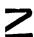
\includegraphics[keepaspectratio]{images/part001_a9d92cc3.jpg}}

Clearly n contains the kernel of this representation. It equals it when M is semi-simple (Proposition 4 (c)), but not in general. It should be noted that an element x of g such that \(x_{M}\) is nilpotent does not necessarily belong to n.

We also note that a particular case of Lemma 3 immediately gives the following result:

PROPOSITION 5. Let \(\mathbf{V}\) be a vector space of finite dimension \(n\) over \(\mathbf{K}\) and \(g\) a Lie subalgebra of \(\mathfrak{gl}(\mathbf{V})\) whose elements are nilpotent endomorphisms of \(\mathbf{V}\) . Then there exists a decreasing sequence of vector subspaces \(\mathrm{V}_0, \mathrm{V}_1, \ldots, \mathrm{V}_n\) of \(\mathbf{V}\) , of dimensions \(n, n - 1, \ldots, 0\) , such that \(x(\mathrm{V}_i) \subset \mathrm{V}_{i+1}\) for all \(x \in g\) and \(i = 0, 1, \ldots, n - 1\) .

\subsection{THE LARGEST NILPOTENT IDEAL OF A LIE ALGEBRA}

Let \(\mathfrak{g}\) be a Lie algebra and \(\mathfrak{a}\) an ideal of \(\mathfrak{g}\) . For \(\mathfrak{a}\) to be nilpotent, it is necessary and sufficient that, for all \(x \in \mathfrak{a}\) , \(\mathrm{ad}_{\mathfrak{g}}x\) be nilpotent; the condition is obviously sufficient and is necessary, for, if \(\mathfrak{a}\) is nilpotent and \(x \in \mathfrak{a}\) , \(\mathrm{ad}_{\mathfrak{a}}x\) is nilpotent and \(\mathrm{ad}_{\mathfrak{a}}x\) maps \(\mathfrak{g}\) into \(\mathfrak{a}\) , hence \(\mathrm{ad}_{\mathfrak{g}}x\) is nilpotent. Then Proposition 4 applied to the adjoint representation of \(\mathfrak{g}\) gives the following result:

PROPOSITION 6. Let \(\mathfrak{g}\) be a Lie algebra and E the associative subalgebra of \(\mathcal{L}(\mathfrak{g})\) generated by 1 and the \(\operatorname{ad}_{\mathfrak{g}}x(x\in \mathfrak{g})\) . Let R be the Jacobson radical of E.

\begin{enumerate}
\def\labelenumi{(\alph{enumi})}
\item
  The set \(\mathfrak{n}\) of \(y\in \mathfrak{g}\) such that \(\operatorname {ad}_{\mathfrak{g}}y\in \mathbb{R}\) is the largest nilpotent ideal of \(\mathfrak{g}\) .
\item
  It is orthogonal to g under the Killing form.
\end{enumerate}

It should be noted that g/n can have non-zero nilpotent ideals.

\subsection{EXTENSION OF THE BASE FIELD}

Let \(\mathfrak{g}\) be a Lie K-algebra, \(\mathrm{K}_1\) an extension of K and \(\mathfrak{g}' = \mathfrak{g}_{(\mathrm{K}_1)}\) . As \(\mathcal{C}^k\mathfrak{g}' = (\mathcal{C}^k\mathfrak{g})_{(\mathrm{K}_1)}\) , \(\mathfrak{g}\) is nilpotent if and only if \(\mathfrak{g}'\) is nilpotent.

Let M be a g-module of finite dimension over K, n the largest nilpotency, ideal for M and \(M' = M_{(K_1)}\) . Let \((\mathrm{M}_i)_{0 \leq i \leq n}\) be a Jordan-Hölder series of the g-module M. Then \(x_{\mathrm{M}}(\mathrm{M}_i) \subset \mathrm{M}_{i+1}\) for all i and all \(x \in n\) , hence

\[
x _ {\mathbf {M} ^ {\prime}} ^ {\prime} \left(\left(\mathrm{M} _ {i}\right) _ {\left(\mathrm{K} _ {1}\right)}\right) \subset \left(\mathrm{M} _ {i + 1}\right) _ {\left(\mathrm{K} _ {1}\right)}
\]

for all \(i\) and all \(x' \in \mathfrak{n}_{(\mathbf{K}_1)}\) ; hence \(x_{\mathbf{M}}'\) is nilpotent for \(x' \in \mathfrak{n}_{(\mathbf{K}_1)}\) , so that \(\mathfrak{n}_{(\mathbf{K}_1)}\) is contained in the largest nilpotency ideal \(\mathfrak{n}'\) for \(\mathbf{M}'\) . We shall now see that, if \(\mathbf{K}_1\) is separable over \(\mathbf{K}\) , then \(\mathfrak{n}' = \mathfrak{n}_{(\mathbf{K}_1)}\) . Let \(\mathbf{E}\) be the associative K-algebra generated by 1 and the \(\mathbf{x}_{\mathbf{M}}\) ( \(x \in \mathfrak{g}\) ), E' the associative K-algebra generated by 1 and the \(\mathbf{x}_{\mathbf{M}}\) ( \(x' \in \mathfrak{g}'\) ) and \(\mathbf{R}\) and \(\mathbf{R}'\) the Jacobson radicals of \(\mathbf{E}\) and \(\mathbf{E}'\) . The algebra E' is canonically identified with \(\mathrm{E}_{(\mathbf{K}_1)}\) . Then \(\mathrm{R}' = \mathrm{R}_{(\mathbf{K}_1)}\) (Algebra, Chapter VIII, § 7, no. 2, Corollary 2 (c) to Proposition 3). Then let \(y' \in \mathfrak{n}'\) and write \(y^{\prime} = \sum_{i = 1}^{n}\lambda_{i}y_{i}\) , where the \(y_{i}\) are in \(\mathfrak{g}\) and the \(\lambda_{i}\in \mathrm{K}_{1}\) are linearly independent over K. Then \(y_{\mathbf{M}'}' = \sum_{i=1}^{n} \lambda_i(y_i)_{\mathbf{M}'}\) and \(y_{\mathbf{M}'}' \in \mathbb{R}' = \mathbb{R}_{(\mathbf{K}_1)}\) . Hence \((y_i)_{\mathbf{M}} \in \mathbb{R}\) and therefore \(y_i \in \mathfrak{n}\) for all \(i\) . It follows that \(y' \in \mathfrak{n}_{(\mathbf{K}_1)}\) , whence \(\mathfrak{n}' \subset \mathfrak{n}_{(\mathbf{K}_1)}\) .

In particular, if \(\mathbf{K}_1\) is separable over \(\mathbf{K}\) , the largest nilpotent ideal of \(\mathfrak{g}_{(\mathbf{K}_1)}\) is derived from that of \(\mathfrak{g}\) by extending the base field from \(\mathbf{K}\) to \(\mathbf{K}_1\) .

\section{SOLVABLE LIE ALGEBRAS}

Recall that K henceforth denotes a field of characteristic 0 and that all Lie algebras are assumed to be finite-dimensional over K.†

\subsection{DEFINITION OF SOLVABLE LIE ALGEBRAS}

DEFINITION 1. A Lie algebra g is called solvable if its kth derived algebra \(\mathcal{D}^{k}\mathfrak{g}\) is zero for sufficiently large \(k\) .

A nilpotent Lie algebra is solvable.

PROPOSITION 1. Subalgebras and quotient algebras of a solvable Lie algebra are solvable. Every extension of a solvable algebra by a solvable algebra is solvable. Every finite product of solvable algebras is solvable.

Let g be a Lie algebra, \(g'\) a subalgebra, h an ideal of g, t = g/h and \(\phi\) the canonical mapping of g onto t. If g is solvable then \(D^{k}g = \{0\}\) for some integer k, hence \(D^{k}g' \subset D^{k}g = \{0\}\) , \(D^{k}t = \phi(\mathcal{D}^{k}g) = \{0\}\) and hence \(g'\) and t are solvable. If h and t are solvable, there exist integers s, t such that

\[
\mathcal {D} ^ {s} \mathfrak {h} = \mathcal {D} ^ {t} \mathfrak {k} = \{0 \};
\]

then \(\mathcal{D}^t\mathfrak{g}\subset \mathfrak{h}\) , hence \(\mathcal{D}^{s + t}\mathfrak{g} = \mathcal{D}^{s}(\mathcal{D}^{t}\mathfrak{g})\subset \mathcal{D}^{s}\mathfrak{h} = \{0\}\) and \(\mathfrak{g}\) is solvable. The last assertion follows from the second by induction on the number of factors.

PROPOSITION 2. Let g be a Lie algebra. The following conditions are equivalent:

\begin{enumerate}
\def\labelenumi{(\alph{enumi})}
\item
  g is solvable;
\item
  there exists a decreasing sequence \(\mathfrak{g} = \mathfrak{g}_0 \supset \mathfrak{g}_1 \supset \dots \supset \mathfrak{g}_n = \{0\}\) of ideals of \(\mathfrak{g}\) such that the algebras \(\mathfrak{g}_i / \mathfrak{g}_{i+1}\) are commutative ( \(i = 0, 1, \ldots, n-1\) );
\item
  there exists a decreasing sequence \(\mathfrak{g} = \mathfrak{g}_0' \supset \mathfrak{g}_1' \supset \dots \supset \mathfrak{g}_p' = \{0\}\) of subalgebras of \(\mathfrak{g}\) such that \(\mathfrak{g}_{i+1}'\) is an ideal of \(\mathfrak{g}_i'\) and \(\mathfrak{g}_i'/\mathfrak{g}_{i+1}'\) is commutative ( \(i = 0, 1, \ldots, p - 1\) );
\item
  there exists a decreasing sequence \(\mathfrak{g} = \mathfrak{g}_0'' \supset \mathfrak{g}_1'' \supset \dots \supset \mathfrak{g}_q'' = \{0\}\) of subalgebras of \(\mathfrak{g}\) such that \(\mathfrak{g}_{i+1}''\) is an ideal of \(\mathfrak{g}_i''\) of codimension 1 ( \(i = 0, 1, \ldots, q - 1\) ).
\item
  \(\Rightarrow\) (b): it suffices to consider the sequence of derived ideals of g.
\item
  \(\Rightarrow\) (c): this is obvious.
\item
  \(\Rightarrow\) (d): suppose that condition (c) holds; every vector subspace of \(\mathfrak{g}_i'\) containing \(\mathfrak{g}_{i+1}'\) is an ideal of \(\mathfrak{g}_i'\) , whence immediately (d).
\item
  \(\Rightarrow\) (a): this follows immediately from the fact that an extension of a solvable algebra by a solvable algebra is solvable.
\end{enumerate}

\subsection*{Examples of solvable Lie algebras}

I. Let g be a 2-dimensional vector space over K and \((e_{1}, e_{2})\) a basis of g. There exists one and only one alternating bilinear multiplication \((x, y) \mapsto [x, y]\) on g such that \([e_{1}, e_{2}] = e_{2}\) . It is easily verified that g is thus given a solvable Lie algebra structure. Now let h be a non-commutative Lie algebra of dimension 2 over K. We show that h is isomorphic to g. Let \((f_{1}, f_{2})\) be a basis of h. The element \([f_{1}, f_{2}]\) is non-zero (otherwise h would be commutative) and hence it generates a 1-dimensional subspace t of h. Then \([h, h] = t\) . Let \((e_{1}^{\prime}, e_{2}^{\prime})\) be a basis of h such that \(e_{2}^{\prime} \in t\) . Then \([e_{1}^{\prime}, e_{2}^{\prime}] = \lambda e_{2}^{\prime}\) with \(\lambda \neq 0\) . Replacing \(e_{1}^{\prime}\) by \(\lambda^{-1}e_{1}\) , it can be assumed that \(\lambda = 1\) , whence our assertion.

\begin{enumerate}
\def\labelenumi{\Roman{enumi}.}
\setcounter{enumi}{1}
\tightlist
\item
  Formulae (5) of §1 prove that \(\mathcal{D}t(n, \mathbf{K}) = \mathfrak{n}(n, \mathbf{K})\) . As \(\mathfrak{n}(n, \mathbf{K})\) is nilpotent and hence solvable, \(t(n, \mathbf{K})\) is solvable. Therefore \(\operatorname{st}(n, \mathbf{K})\) is solvable. In particular, \(\operatorname{st}(2, \mathbf{K})\) is isomorphic to the algebra of Example I.
\end{enumerate}

\subsection{RADICAL OF A LIE ALGEBRA}

Let \(a, b\) be two solvable ideals of a Lie algebra \(g\) . The algebra \((a + b)/b\) is isomorphic to \(a/(a \cap b)\) and hence is solvable and \(a + b\) , which is an extension of \((a + b)/b\) by \(b\) , is also solvable (Proposition 1). It follows that a maximal solvable ideal of \(g\) contains every solvable ideal of \(g\) and hence \(g\) has a largest solvable ideal. This enables us to make the following definition:

DEFINITION 2. The radical of a Lie algebra is its largest solvable ideal.

PROPOSITION 3. The radical \(\mathfrak{r}\) of a Lie algebra \(\mathfrak{g}\) is the smallest ideal of \(\mathfrak{g}\) such that \(\mathfrak{g} / \mathfrak{r}\) has radical \(\{0\}\) .

Let \(\mathfrak{a}\) be an ideal of \(\mathfrak{g}\) and \(\phi\) the canonical mapping of \(\mathfrak{g}\) onto \(\mathfrak{g}/\mathfrak{a}\) . If the radical of \(\mathfrak{g}/\mathfrak{a}\) is zero, then \(\phi(\mathfrak{r})\) , which is a solvable ideal of \(\mathfrak{g}/\mathfrak{a}\) , is zero; hence \(\mathfrak{r} \subset \mathfrak{a}\) . On the other hand, the inverse image \(\overline{\phi}^{-1}(\mathfrak{r}')\) of the radical \(\mathfrak{r}'\) of \(\mathfrak{g}/\mathfrak{r}\) is an ideal of \(\mathfrak{g}\) which is solvable by Proposition 1 and hence is equal to \(\mathfrak{r}\) ; therefore \(\mathfrak{r}' = \{0\}\) .

PROPOSITION 4. Let \(\mathfrak{g}_1, \ldots, \mathfrak{g}_n\) be Lie algebras. The radical \(\mathfrak{r}\) of the product of the \(\mathfrak{g}_i\) is the product of the radicals \(\mathfrak{r}_i\) of the \(\mathfrak{g}_i\) .

The product \(\mathfrak{r}'\) of the \(\mathfrak{r}_i\) is a solvable ideal (Proposition 1) and hence \(\mathfrak{r}' \subset \mathfrak{r}\) . The canonical image of \(\mathfrak{r}\) in \(\mathfrak{g}_i\) is a solvable ideal of \(\mathfrak{g}_i\) and hence is contained in \(\mathfrak{r}_i\) ; hence \(\mathfrak{r} \subset \mathfrak{r}'\) .

\subsection{NILPOTENT RADICAL OF A LIE ALGEBRA}

DEFINITION 3. Let g be a Lie algebra. The nilpotent radical of g is the intersection of the kernels of the finite-dimensional simple representations of g.

Remarks. (1) Let \(\mathfrak{s}\) be the nilpotent radical of \(\mathfrak{g}\) . As every decreasing sequence of vector subspaces of \(\mathfrak{g}\) is stationary, there exists a finite number of finite-dimensional simple representations of \(\mathfrak{g}\) whose kernels have intersection \(\mathfrak{s}\) .

The direct sum of these representations is semi-simple and has kernel s. It follows that the set of kernels of finite-dimensional semi-simple representations of g has a least element, namely s.

\begin{enumerate}
\def\labelenumi{(\arabic{enumi})}
\setcounter{enumi}{1}
\item
  By Proposition 4 (c) of §4, no. 3, s is also the intersection of the largest nilpotency ideals of the finite-dimensional representations of g. In particular, s is contained in the largest nilpotent ideal of g and is therefore a nilpotent ideal of g.
\item
  Every linear form \(\lambda\) on \(\mathfrak{g}\) which is zero on \(\mathcal{D}\mathfrak{g}\) is a simple representation (with space \(\mathbf{K}\) ) of \(\mathfrak{g}\) , whence \(\lambda (\mathfrak{s}) = \{0\}\) . It follows that \(\mathfrak{s} \subset \mathcal{D}\mathfrak{g}\) . On the other hand, \(\mathfrak{s}\) is contained in the radical \(\mathfrak{r}\) of \(\mathfrak{g}\) by Remark 2. We shall prove that \(\mathfrak{s} = \mathfrak{r} \cap \mathcal{D}\mathfrak{g}\) .
\end{enumerate}

Lemma 1. Let \(\mathbf{V}\) be a finite-dimensional vector space over \(\mathbf{K}\) , \(\mathfrak{g}\) a subalgebra of \(\mathfrak{gl}(\mathbf{V})\) such that \(\mathbf{V}\) is a simple \(\mathfrak{g}\) -module and \(\mathfrak{a}\) a commutative ideal of \(\mathfrak{g}\) . Then \(\mathfrak{a} \cap \mathcal{D}\mathfrak{g} = \{0\}\) . Let \(\mathbf{S}\) be the subalgebra of \(\mathcal{L}(\mathbf{V})\) generated by 1 and \(\mathfrak{a}\) .

If \(\mathfrak{b}\) is an ideal of \(\mathfrak{g}\) contained in \(\mathfrak{a}\) such that \(\operatorname{Tr}bs = 0\) for all \(b\in \mathfrak{b}\) and all \(s\in S\) , then in particular, by definition of \(S\) , \(\operatorname{Tr}(b^n) = 0\) for every integer \(n > 0\) and hence \(b\) is nilpotent (Algebra, Chapter VII, § 5, no. 5, Corollary 4 to Proposition 13); as the elements of \(\mathfrak{b}\) are all nilpotent, \(\mathfrak{b} = \{0\}\) (§ 4, no. 3, Lemma 2). We first apply this to the ideal \([\mathfrak{g},\mathfrak{a}]\) of \(\mathfrak{g}\) . If \(x\in \mathfrak{g}\) , \(a\in \mathfrak{a}\) , \(s\in S\) , then \(\operatorname{Tr}[x,a]s = \operatorname{Tr}(xas - axs) = \operatorname{Tr}x(as - sa) = 0\) since \(as = sa\) ; hence \([\mathfrak{g},\mathfrak{a}] = \{0\}\) . Hence the elements of \(\mathfrak{g}\) commute with those of \(\mathfrak{a}\) and hence also with those of \(S\) . If \(x,y\) belong to \(\mathfrak{g}\) and \(s\in S\) , then

\[
\operatorname{Tr} [ x, y ] s = \operatorname{Tr} (x y s - y x s) = \operatorname{Tr} x (y s - s y) = 0
\]

since \(ys = sy\) ; then taking \(b\) to be the ideal \(\mathcal{D}\mathfrak{g} \cap a\) , it follows that \(\mathcal{D}\mathfrak{g} \cap a = \{0\}\) .

THEOREM 1. Let \(\mathfrak{g}\) be a Lie algebra, \(\mathfrak{r}\) its radical and \(\mathfrak{s}\) its nilpotent radical. Then \(\mathfrak{s} = \mathcal{D}\mathfrak{g} \cap \mathfrak{r}\) .

We already know that \(\mathfrak{s} \subset \mathcal{D}\mathfrak{g} \cap \mathfrak{r}\) . Hence it will suffice to show that if \(\rho\) is a finite-dimensional simple representation of \(\mathfrak{g}\) then \(\rho(\mathcal{D}\mathfrak{g} \cap \mathfrak{r}) = \{0\}\) . Let \(k\) be the least integer \(\geqslant 0\) such that \(\rho(\mathcal{D}^{k}\mathfrak{r}) = \{0\}\) ; we write \(\mathfrak{g}' = \rho(\mathfrak{g})\) , \(\mathfrak{a}' = \rho(\mathrm{D}^k\mathfrak{r})\) ; as \(\mathcal{D}^k\mathfrak{r}\) is an ideal of \(\mathfrak{g}\) , \(\mathfrak{a}'\) is an ideal of \(\mathfrak{g}'\) ; this ideal is commutative since \(\rho(\mathcal{D}^{k}\mathfrak{r}) = \{0\}\) . If \(\mathrm{V}\) is the space of \(\rho\) , \(\mathfrak{g}' \subset \mathfrak{gl}(\mathrm{V})\) and \(\mathrm{V}\) is a simple \(\mathfrak{g}'\) -module. Then \(\rho(\mathcal{D}\mathfrak{g} \cap \mathcal{D}^k\mathfrak{r}) \subset \mathcal{D}\mathfrak{g}' \cap \mathfrak{a}' = \{0\}\) . If \(k > 0\) , then \(\mathcal{D}^k\mathfrak{r} \subset \mathcal{D}\mathfrak{g}\) and \(\rho(\mathcal{D}^k\mathfrak{r}) = \{0\}\) , contrary to the definition of \(k\) . Hence \(k = 0\) , that is

\[
\rho (\mathcal{D}\mathfrak{g} \cap \mathfrak{r}) = \{0 \}.
\]

COROLLARY 1. Let g be a solvable Lie algebra. The nilpotent radical of g is \(\mathcal{D}\mathfrak{g}\) . If \(\rho\) is a finite-dimensional simple representation of g, \(\rho(\mathfrak{g})\) is commutative and the associative algebra L generated by 1 and \(\rho(\mathfrak{g})\) is a field of finite degree over K.

Here \(\mathfrak{r} = \mathfrak{g}\) , whence \(\mathfrak{s} = \mathcal{D}\mathfrak{g}\) . Hence \(\rho(\mathcal{D}\mathfrak{g}) = \{0\}\) , which shows that \(\mathfrak{g}' = \rho(\mathfrak{g})\) is commutative. Every element \(\neq 0\) of \(\mathbf{L}\) is invertible by Schur's Lemma; hence \(\mathbf{L}\) is a field.

COROLLARY 2 (Lie's Theorem). Let \(\mathfrak{g}\) be a solvable Lie algebra; suppose that \(\mathbf{K}\) is algebraically closed. Let \(\mathbf{M}\) be a \(\mathfrak{g}\) -module of finite dimension over \(\mathbf{K}\) and let \((\mathrm{M}_1)_{0 \leqslant i \leqslant r}\) be a Jordan-Hölder series of \(\mathbf{M}\) . Then \(\mathrm{M}_{i - 1} / \mathrm{M}_i\) is of dimension 1 over \(\mathbf{K}\) for \(1 \leqslant i \leqslant r\) and, for all \(x \in \mathfrak{g}\) , \(x_{\mathrm{M}_{i - 1} / \mathrm{M}_i} = \lambda_i(x)\) . 1, where \(\lambda_i\) is a linear form on \(\mathfrak{g}\) which is zero on \(\mathcal{D}\mathfrak{g}\) . In particular, every simple \(\mathfrak{g}\) -module of finite dimension over \(\mathbf{K}\) is in fact of dimension 1.

Let \(\rho_{i}\) be the representation of \(g\) on \(\mathbf{M}_{i-1}/\mathbf{M}_{i}\) . The associative algebra \(\mathbf{L}_{i}\) generated by 1 and \(\rho_{i}(g)\) is a field, a finite extension of K and therefore equal to K; and \(\mathbf{M}_{i-1}/\mathbf{M}_{i}\) is a simple \(\mathbf{L}_{i}\) -module, whence \(\dim \mathbf{M}_{i-1}/\mathbf{M}_{i} = 1\) . The rest of the corollary is obvious.

Remarks. (1) If \((\mathrm{M}_i)_{0\leqslant i\leqslant r}\) is replaced by another Jordan-Hölder series of M, the sequence \((\lambda_1,\dots ,\lambda_r)\) is replaced by a sequence of the form \((\lambda_{\pi (1)},\dots ,\lambda_{\pi (r)})\) where \(\pi\) is a permutation of \(\{1,\dots ,r\}\) , as follows from the Jordan-Hölder Theorem.

\begin{enumerate}
\def\labelenumi{(\arabic{enumi})}
\setcounter{enumi}{1}
\tightlist
\item
  Let \((e_1, \ldots, e_r)\) be a basis of M such that \(e_i \in \mathbf{M}_{i-1}, e_i \notin \mathbf{M}_i\) ( \(1 \leqslant i \leqslant r\) ). If \(x \in \mathfrak{g}\) the endomorphism of M corresponding to \(x\) is represented with respect to this basis by a triangular matrix whose diagonal coefficients are
\end{enumerate}

\[
\lambda_ {1} (x), \dots , \lambda_ {\tau} (x).
\]

COROLLARY 3. Suppose that K is algebraically closed. If g is an r-dimensional solvable Lie algebra, every ideal of g is a term of a decreasing sequence of ideals of dimensions r, r - 1, \ldots, 0.

Every ideal is part of a Jordan-Hölder series of g, considered as the space of the adjoint representation (Algebra, Chapter I, § 6, no. 14, Corollary to Theorem 8); then it suffices to apply Corollary 2.

COROLLARY 4. Suppose that \(\mathbf{K} = \mathbf{R}\) . Let \(\mathfrak{g}\) be a solvable Lie algebra. Every simple representation of \(\mathfrak{g}\) is of dimension \(\leqslant 2\) . Every ideal of \(\mathfrak{g}\) is a term of a decreasing sequence \((\mathfrak{g}_i)_{0\leqslant i\leqslant m}\) of ideals such that \(\mathfrak{g}_0 = \mathfrak{g},\mathfrak{g}_m = \{0\}\) , \(\dim \mathfrak{g}_{i - 1} / \mathfrak{g}_i\leqslant 2\) ( \(1\leqslant i\leqslant m\) ).

This is proved in a similar way to that for Corollaries 2 and 3, using the fact that every algebraic extension of \(\mathbf{R}\) is of degree \(\leqslant 2\) .

COROLLARY 5. For a Lie algebra g to be solvable, it is necessary and sufficient that \(\mathcal{D}\mathfrak{g}\) be nilpotent.

The condition is necessary by Corollary 1. It is sufficient since \(\mathfrak{g} / \mathcal{D}\mathfrak{g}\) is commutative.

COROLLARY 6. Let \(\rho\) be a finite-dimensional representation of a Lie algebra \(\mathfrak{g}\) . Let \(\mathfrak{r}\) be the radical of \(\mathfrak{g}\) . Every element \(x \in \mathfrak{r}\) such that \(\rho(x)\) is nilpotent belongs to the largest nilpotency ideal \(\mathfrak{n}\) of \(\rho\) .

Let \(V\) be the space of \(\rho\) ; let \(\langle V_i \rangle_{0 \leqslant i \leqslant r}\) be a Jordan-Hölder series for the \(r\) -module structure on \(V\) and let \(\rho_i\) be the representation of \(r\) with space \(V_i / V_{i-1}\) ( \(1 \leqslant i \leqslant r\) ). If \(\rho(x)\) is nilpotent, so is \(\rho_i(x)\) ; as for all \(i\) the algebra generated by \(\rho_i(x)\) is a field, \(\rho_i(x) = 0\) . Conversely, if \(\rho_i(x) = 0\) for all \(i, \rho(x) = 0\) . This shows that the set \(a\) of \(x \in r\) such that \(\rho(x)\) is nilpotent is an ideal of \(r\) . On the other hand, \([g, a] \subset \mathcal{D}g \cap r \subset n \cap r \subset a\) and hence \(a\) is an ideal of \(g\) . This proves that \(a \subset n\) .

COROLLARY 7. Let g be a Lie algebra and r its radical. The following four sets are identical: (a) the largest nilpotent ideal of g; (b) the largest nilpotent ideal of r; (c) the set of \(x \in \mathfrak{r}\) such that \(\operatorname{ad}_{\mathfrak{g}} x\) is nilpotent; (d) the set of \(x \in \mathfrak{r}\) such that \(\operatorname{ad}_{\mathfrak{r}} x\) is nilpotent.

Let these sets be denoted by \(\mathfrak{a}, \mathfrak{b}, \mathfrak{c}, \mathfrak{d}\) . The inclusions \(\mathfrak{a} \subset \mathfrak{b} \subset \mathfrak{d} \subset \mathfrak{c}\) are clear. \(\mathfrak{c} \subset \mathfrak{a}\) by Corollary 6 applied to the adjoint representation of \(\mathfrak{g}\) .

\subsection{A CRITERION FOR SOLVABILITY}

Lemma 2. Let \(x\) be an endomorphism of a finite-dimensional vector space \(V\) and \(s\) (resp. \(n\) ) its semi-simple (resp. nilpotent) component (cf.~Algebra, Chapter VIII, § 9, no. 4, Definition 4). Let \(ad_x\) , \(ad_s\) , \(ad_n\) be the respective images of \(x\) , \(s\) , \(n\) in the adjoint representation of \(gl(V)\) . Then \(ad_s\) (resp. \(ad_n\) ) is the semi-simple (resp. nilpotent) component of \(ad_x\) and is equal to a polynomial in \(ad_x\) with coefficients in \(K\) and no constant term.

We know that \(\operatorname{ad} x = \operatorname{ad} s + \operatorname{ad} n\) , \([\operatorname{ad} s, \operatorname{ad} n] = 0\) and \(\operatorname{ad} n\) is nilpotent (§ 4, Lemma 1). We show that \(\operatorname{ad} s\) is semi-simple. It suffices to do this when \(\mathbf{K}\) is algebraically closed (cf.~Algebra, Chapter VIII, § 9, no. 2, Proposition 3). Then let \((e_i)_{1 \leq i \leq n}\) be a basis of \(V\) such that \(s(e_i) = \lambda_i e_i\) ( \(\lambda_i \in K\) ). Let \((E_{ij})\) be the canonical basis of \(\mathbf{M}_n(K) = \mathfrak{gl}(V)\) . By formulae (5) of § 1,

\[
(\mathrm{ad} s). E _ {i j} = (\lambda_ {i} - \lambda_ {j}) E _ {i j}
\]

and hence ad s is semi-simple. The last assertion of the lemma follows from Algebra, Chapter VIII, § 9, no. 4, Proposition 8.

Lemma 3. Let \(\mathbf{M}\) be a finite-dimensional vector space, \(\mathbf{A}\) and \(\mathbf{B}\) two vector subspaces of \(\mathfrak{gl}(\mathbf{M})\) such that \(\mathbf{B} \subset \mathbf{A}\) and \(\mathbf{T}\) the set of \(t \in \mathfrak{gl}(\mathbf{M})\) such that \([t, \mathbf{A}] \subset \mathbf{B}\) . If \(z \in \mathbf{T}\) is such that \(\operatorname{Tr}(zu) = 0\) for all \(u \in \mathbf{T}\) , then \(z\) is nilpotent.

It suffices to prove this when \(\mathbf{K}\) is algebraically closed, which we shall assume henceforth. Let \(s\) and \(n\) be the semi-simple and nilpotent components of \(z\) and let \((e_i)\) be a basis of \(\mathbf{M}\) such that \(s(e_i) = \lambda_i e_i\) ( \(\lambda_i \in \mathbf{K}\) ). Let \(\mathbf{V} \subset \mathbf{K}\) be the vector space over \(\mathbf{Q}\) generated by the \(\lambda_i\) . We need to prove that \(\mathbf{V} = \{0\}\) . Let \(f\) be a \(\mathbf{Q}\) -linear form on \(\mathbf{V}\) and let \(t\) be the endomorphism of \(\mathbf{M}\) such that \(te_{i}=f(\lambda_{i})e_{i}\) . If \((E_{ij})\) is the canonical basis of gl(M) defined by \(E_{ij}e_{k}=\delta_{jk}e_{i}\) , then

\[
\begin{array}{l} (\mathrm{ad} s) E _ {i j} = (\lambda_ {i} - \lambda_ {j}) E _ {i j} \\ (\mathrm{ad} t) E _ {i j} = (f (\lambda_ {i}) - f (\lambda_ {j})) E _ {i j}. \end{array}
\]

There exists a polynomial \(\mathbf{P}\) with no constant term and with coefficients in \(\mathbf{K}\) such that \(\mathrm{P}(\lambda_i - \lambda_j) = f(\lambda_i) - f(\lambda_j)\) for all \(i\) and \(j\) (for if \(\lambda_i - \lambda_j = \lambda_h - \lambda_k\) , then \(f(\lambda_i) - f(\lambda_j) = f(\lambda_h) - f(\lambda_k)\) ) and, if \(\lambda_i - \lambda_j = 0\) , \(f(\lambda_i) - f(\lambda_j) = 0\) ). Then ad \(t = \mathrm{P}(\mathrm{ad}s)\) . On the other hand, ad \(s\) is a polynomial with no constant term in ad \(z\) . Now (ad \(z\) ) (A) \(\subset \mathrm{B}\) , whence also (ad \(t\) ) (A) \(\subset \mathrm{B}\) . By the hypothesis \(0 = \operatorname{Tr}(zt) = \sum_{\lambda_i} f(\lambda_i)\) , whence \(0 = f(\operatorname{Tr}(zt)) = \sum f(\lambda_i)^2\) . Since the \(f(\lambda_i)\) are rational numbers, \(f = 0\) , which completes the proof.

THEOREM 2 (Cartan's criterion). Let \(\mathfrak{g}\) be a Lie algebra, \(\mathbf{M}\) a finite-dimensional vector space, \(\rho\) a representation of \(\mathfrak{g}\) on \(\mathbf{M}\) and \(\beta\) the bilinear form on \(\mathfrak{g}\) associated with \(\rho\) . Then \(\rho(\mathfrak{g})\) is solvable if and only if \(\mathcal{D}\mathfrak{g}\) is orthogonal to \(\mathfrak{g}\) with respect to \(\beta\) .

It can obviously be reduced to the case where \(\mathfrak{g}\) is a Lie subalgebra of \(\mathfrak{gl}(\mathbf{M})\) and \(\rho\) is the identity mapping. If \(\mathfrak{g}\) is solvable, \(\mathcal{D}\mathfrak{g}\) is contained in the largest nilpotency ideal of the identity representation of \(\mathfrak{g}\) (Theorem 1) and hence is orthogonal to \(\mathfrak{g}\) with respect to \(\beta\) ( \(\S 4\) , Proposition 4 (d)). Suppose that \(\mathcal{D}\mathfrak{g}\) is orthogonal to \(\mathfrak{g}\) with respect to \(\beta\) . We prove that \(\mathfrak{g}\) is solvable. Let \(\mathrm{T}\) be the set of \(t\in \mathfrak{gl}(\mathbf{M})\) such that \([t,\mathfrak{g}]\subset \mathcal{D}\mathfrak{g}\) . If \(t\in \mathrm{T}\) and \(x,y\) belong to \(\mathfrak{g}\) , then \([t,x]\in \mathcal{D}\mathfrak{g}\) and hence

\[
\operatorname{Tr} (t [ x, y ]) = \beta ([ t, x ], y) = 0
\]

whence by linearity \(\mathrm{Tr}(tu) = 0\) for all \(u\in \mathcal{D}\mathfrak{g}\) . Also, clearly \(\mathcal{D}\mathfrak{g}\subset T\) . Hence (Lemma 3) every element of \(\mathcal{D}\mathfrak{g}\) is nilpotent. It follows that \(\mathcal{D}\mathfrak{g}\) is nilpotent (§ 4, Corollary 3 to Theorem 1) and hence that \(\mathfrak{g}\) is solvable (no. 3, Corollary 5 to Theorem 1).

\subsection{FURTHER PROPERTIES OF THE RADICAL}

PROPOSITION 5. Let g be a Lie algebra and r its radical.

\begin{enumerate}
\def\labelenumi{(\alph{enumi})}
\item
  If \(\rho\) is a finite-dimensional representation of \(\mathfrak{g}\) and \(\beta\) is the associated bilinear form, \(\mathfrak{r}\) and \(\mathcal{D}\mathfrak{g}\) are orthogonal with respect to \(\beta\) .
\item
  r is the orthogonal of \(\mathcal{D}\mathfrak{g}\) with respect to the Killing form.
\end{enumerate}

Let \(x, y\) be in \(\mathfrak{g}, z \in \mathfrak{r}\) . Then \([y, z] \in \mathcal{D}\mathfrak{g} \cap \mathfrak{r}\) and hence

\[
\beta ([ x, y ], z) = \beta (x, [ y, z ]) = 0
\]

(Theorem 1). Hence (a).

Let \(\mathfrak{r}'\) be the orthogonal of \(\mathcal{D}\mathfrak{g}\) with respect to the Killing form. It is an ideal of \(\mathfrak{g}\) ( \(\S 3\) , no. 6, Proposition 7 (a)) which contains \(\mathfrak{r}\) by the above. On the other hand, the image s of \(\mathfrak{r}'\) under the adjoint representation of \(\mathfrak{g}\) is solvable (Theorem 2) and hence \(\mathfrak{r}'\) is solvable being a central extension of s. Hence \(\mathfrak{r}' \subset \mathfrak{r}\) .

COROLLARY 1. Let \(\mathfrak{g}\) be a Lie algebra. Then \(\mathfrak{g}\) is solvable if and only if \(\mathcal{D}\mathfrak{g}\) is orthogonal to \(\mathfrak{g}\) with respect to the Killing form.

This is an immediate consequence of Proposition 5 (b).

COROLLARY 2. The radical \(\mathfrak{r}\) of a Lie algebra \(\mathfrak{g}\) is a characteristic ideal.

\(\mathcal{D}\mathfrak{g}\) is a characteristic ideal and the Killing form is completely invariant (§ 3, no. 6, Proposition 10). Hence the orthogonal of \(\mathcal{D}\mathfrak{g}\) with respect to the Killing form is a characteristic ideal (§ 3, no. 6, Proposition 7 (b)).

COROLLARY 3. Let g be a Lie algebra, r its radical and a an ideal of g. Then the radical of a is equal to r ∩ a.

\(r \cap a\) is a solvable ideal of \(a\) and hence is contained in the radical \(r'\) of \(a\) . Conversely, \(r'\) is an ideal of \(g\) (Corollary 2 and §1, no. 4, Proposition 2) and hence \(r' \subset r\) .

Corollary 2 can be made more precise as follows:

PROPOSITION 6. Let \(\mathfrak{g}\) be a Lie algebra, \(\mathfrak{r}\) its radical and \(\mathfrak{n}\) its largest nilpotent ideal. Every derivation of \(\mathfrak{g}\) maps \(\mathfrak{r}\) into \(\mathfrak{n}\) .

Let D be a derivation of g. Let \(g' = g + Kx_0\) be a Lie algebra in which g is an ideal of codimension 1 such that \(Dx = [x_0, x]\) for all \(x \in g\) (§ 1, no. 8, Example 1). By Corollary 3 to Proposition 5, r is contained in the radical \(r'\) of \(g'\) . Then \(D(r) = [x_0, r] \subset [g', g'] \cap r' = s'\) . For all \(x \in s' \cup g\) , \(ad_g x\) is nilpotent (Theorem 1). Hence, for all \(x \in s' \cap g\) , \(ad_g x\) is nilpotent. Hence \(D(r)\) is contained in the nilpotent ideal \(s' \cap g\) of g.

COROLLARY. The largest nilpotent ideal of a Lie algebra is a characteristic ideal.

Remark. To summarize some of the above results, note that, if r, n, s, t denote respectively the radical of g, the largest nilpotent ideal of g, the nilpotent radical of g and the orthogonal of g with respect to the Killing form, then

\[
\mathfrak {r} \supset \mathfrak {k} \supset \mathfrak {n} \supset \mathfrak {s}.
\]

The inclusion \(\mathfrak{r} \supset \mathfrak{t}\) follows from Proposition 5 (b). The inclusion \(\mathfrak{t} \supset \mathfrak{n}\) follows from §4, no. 4, Proposition 6 (b). The inclusion \(\mathfrak{n} \supset \mathfrak{s}\) has been pointed out in Remark 2 of no. 3.

\subsection{EXTENSION OF THE BASE FIELD}

Let \(\mathfrak{g}\) be a Lie K-algebra and \(\mathbf{K}_1\) an extension of K. Clearly \(\mathfrak{g}_{(\mathbf{K}_1)}\) is solvable if and only if \(\mathfrak{g}\) is solvable, since \(\mathcal{D}^n (\mathfrak{g}_{(\mathbf{K}_1)}) = (\mathcal{D}^n\mathfrak{g})_{(\mathbf{K}_1)}\) .

Let \(\mathfrak{r}\) be the radical of \(\mathfrak{g}\) . Then \(\mathfrak{r}_{(\mathbf{K}_1)}\) is the radical of \(\mathfrak{g}_{(\mathbf{K}_1)}\) . For let \(\beta\) be the Killing form of \(\mathfrak{g}\) . As \(\mathfrak{r}\) is the orthogonal of \(\mathcal{D}\mathfrak{g}\) with respect to \(\beta\) (Proposition 5 (b)), \(\mathfrak{r}_{(\mathbf{K}_1)}\) is the orthogonal of \((\mathcal{D}\mathfrak{g})_{(\mathbf{K}_1)} = \mathcal{D}(\mathfrak{g}_{(\mathbf{K}_1)})\) with respect to the form derived from \(\beta\) by extension from \(\mathbf{K}\) to \(\mathbf{K}_1\) , that is the Killing form of \(\mathfrak{g}_{(\mathbf{K}_1)}\) ( \(\S 3\) , no. 8). Our assertion then follows from a further application of Proposition 5 (b).

\section{SEMI-SIMPLE LIE ALGEBRAS}

Recall that K denotes a field of characteristic 0 and that all Lie algebras are assumed to be finite-dimensional over K.

\subsection{DEFINITION OF SEMI-SIMPLE LIE ALGEBRAS}

DEFINITION 1. Let \(\mathfrak{g}\) be a Lie algebra. \(\mathfrak{g}\) is called semi-simple if and only if the only commutative ideal of \(\mathfrak{g}\) is \(\{0\}\) .

Remarks. (1) The algebra \(\{0\}\) is semi-simple. An algebra of dimension 1 or 2 is not semi-simple (cf.~§ 5, no. 1, Example 1). There exist semi-simple algebras of dimension 3 (cf.~no. 7).

\begin{enumerate}
\def\labelenumi{(\arabic{enumi})}
\setcounter{enumi}{1}
\item
  A semi-simple algebra has zero centre and hence its adjoint representation is faithful.
\item
  If \(g_{1}, \ldots, g_{n}\) are semi-simple, \(g = g_{1} \times \cdots \times g_{n}\) is semi-simple: for if a is a commutative ideal of g, the projections of a onto \(g_{1}, \ldots, g_{n}\) reduce to \(\{0\}\) .
\end{enumerate}

THEOREM 1. Let \(\mathfrak{g}\) be a Lie algebra. The following conditions are equivalent:

\begin{enumerate}
\def\labelenumi{(\alph{enumi})}
\item
  g is semi-simple.
\item
  The radical r of g is zero.
\item
  The Killing form \(\beta\) of \(\mathfrak{g}\) is non-degenerate.
\end{enumerate}

Moreover, a semi-simple Lie algebra is equal to its derived ideal.

\begin{enumerate}
\def\labelenumi{(\alph{enumi})}
\item
  \(\Rightarrow\) (b): for if \(\mathfrak{r} \neq \{0\}\) , the last non-zero derived algebra of \(\mathfrak{r}\) is a commutative ideal of \(\mathfrak{g}\) .
\item
  \(\Rightarrow\) (c): this follows from Proposition 5 (b) of § 5, no. 5 (which at the same time proves the last assertion of the theorem).
\item
  \(\Rightarrow\) (a): this follows from Proposition 6 (b) of §4, no. 4.
\end{enumerate}

COROLLARY. Let \(\mathfrak{g}\) be a semi-simple Lie algebra and \(\rho\) a representation of \(\mathfrak{g}\) on a finite-dimensional vector space V. Then \(\rho(\mathfrak{g}) \subset \mathfrak{sl}(V)\) .

The linear form \(x \mapsto \operatorname{Tr} \rho(x)\) ( \(x \in \mathfrak{g}\) ) is zero when \(x\) is of the form \([y, z]\) ( \(y \in \mathfrak{g}, z \in \mathfrak{g}\) ) and hence on \(\mathcal{D}\mathfrak{g} = \mathfrak{g}\) .

PROPOSITION 1. Let \(\mathfrak{g}\) be a semi-simple Lie algebra and \(\rho\) a finite-dimensional faithful representation of \(\mathfrak{g}\) . Then the bilinear form on \(\mathfrak{g}\) associated with \(\rho\) is non-degenerate.

The orthogonal of g with respect to this form is a solvable ideal (§ 5, no. 4, Theorem 2) and hence is zero.

COROLLARY 1. Let g be a Lie algebra, \(\beta\) its Killing form and \(\mathfrak{a}\) a semi-simple subalgebra of g. The orthogonal \(\mathfrak{b}\) of \(\mathfrak{a}\) with respect to \(\beta\) is a supplementary subspace of \(\mathfrak{a}\) in g and \({[}\mathfrak{a}, \mathfrak{b}{]} \subset \mathfrak{b}\). If \(\mathfrak{a}\) is an ideal of g, so is \(\mathfrak{b}\), which is then the centralizer of \(\mathfrak{a}\) in g.

Let \(\beta'\) be the restriction of \(\beta\) to \(a\) : it is the bilinear form associated with the representation \(x \mapsto \operatorname{ad}_{\mathfrak{g}} x\) of \(a\) on the space \(\mathfrak{g}\) . This representation is faithful and hence \(\beta'\) is non-degenerate (Proposition 1). Hence \(\mathfrak{b}\) is supplementary to \(a\) in \(\mathfrak{g}\) . On the other hand, if \(x, y\) are in \(a\) and \(z \in \mathfrak{b}\) , then

\[
\beta (x, [ y, z ]) = \beta ([ x, y ], z) = 0,
\]

 since \([x,y] \in \mathfrak{a}\) , and hence \([y,z] \in \mathfrak{b}\) , which proves that \([\mathfrak{a},\mathfrak{b}] \subset \mathfrak{b}\) . If \(\mathfrak{a}\) is an ideal of \(\mathfrak{g}\) , we know that \(\mathfrak{b}\) is an ideal of \(\mathfrak{g}\) (§ 3, Proposition 7) and \(\mathfrak{g}\) is identified with \(\mathfrak{a} \times \mathfrak{b}\) . As the centre of \(\mathfrak{a}\) is zero, the centralizer of \(\mathfrak{a}\) in \(\mathfrak{g}\) is \(\mathfrak{b}\) .

COROLLARY 2. Every extension of a semi-simple Lie algebra by a semi-simple Lie algebra is semi-simple and trivial.

This follows immediately from Corollary 1.

COROLLARY 3. If g is semi-simple, every derivation of g is inner.

ad g is isomorphic to g and hence semi-simple and is an ideal of the Lie algebra d of derivations of g (§ 1, Proposition 1). If D ∈ d commutes with the elements of ad g, then, for all x ∈ g, ad D(x) = {[}D, ad x{]} = 0, whence D(x) = 0; hence D = 0. Corollary 3 then follows from Corollary 1.
